% \documentclass[aspectratio=43]{beamer}
% \documentclass[aspectratio=169]{beamer}
% \documentclass[handout,aspectratio=43]{beamer}
\documentclass[handout,aspectratio=169]{beamer}

%%%%%%%%%%%%%%%%%%%%%%%%%%%%%%%%%%%%
% Header                           %
%%%%%%%%%%%%%%%%%%%%%%%%%%%%%%%%%%%%
%
% Compilation:
%
% - with pdfLaTeX:
%   pdflatex -> biber -> makeindex/create_glossaries.cmd -> pdflatex -> pdflatex
% - For compilation add switch -shell-escape in your LaTeX editor:
%   pdflatex --shell-escape -synctex=1 -interaction=nonstopmode %source --extra-mem-top=60000000
% - Compile at least 3 times for proper output
%
% In case of problems:
%
% - Increase Tex-Memory in batch with:
%   initexmf --edit-config-file pdflatex
%   add: main_memory=12000000
%   initexmf --dump=pdflatex
%
% Revisions: 2017-04-10 Martin Rädel <martin.raedel@dlr.de>
%                       Initial draft
% 
% Contact:   Martin Rädel,  martin.raedel@dlr.de
%            DLR Composite Structures and Adaptive Systems
%
%                                 __/|__
%                                /_/_/_/  
%            www.dlr.de/fa/en      |/ DLR
%
%%%%%%%%%%%%%%%%%%%%%%%%%%%%%%%%%%%%
% Preamble                         %
%%%%%%%%%%%%%%%%%%%%%%%%%%%%%%%%%%%%

% ---------------------------
% Path to common
% ---------------------------

\newcommand{\peridoccommonpath}{../../../../Doc/PeriDoX_Common}
\newcommand{\peridocliteraturepath}{../../../../Literature}
\newcommand{\materialpath}{../../Material}

% ---------------------------
% Local packages
% ---------------------------

\usepackage[
  style=numeric-comp,
  sorting=none,
  url=false,
  isbn=false
]{biblatex}
\usepackage{booktabs}
\usepackage{caption}
\usepackage{enumitem}
\usepackage{filecontents}
\usepackage{multirow}
% \usepackage{placeins} % for \FloatBarrier
\usepackage{siunitx}
\sisetup{%
  exponent-product = \cdot,%
  output-product = \cdot,%
  separate-uncertainty=true,% uncertainty is separated with a "plus-minus" symbol
}
\usepackage{subcaption}
\usepackage{tabularx}

% General preamble
% %%%%%%%%%%%%%%%%%%%%%%%%%%%%%%%%%%%%
% Header                           %
%%%%%%%%%%%%%%%%%%%%%%%%%%%%%%%%%%%%
% 
% This file handles all things with general packages
% 
% Revisions: 2017-04-10 Martin Raedel <martin.raedel@dlr.de>
%                       Initial draft
%               
% Contact:   Martin Raedel,  martin.raedel@dlr.de
%            DLR Composite Structures and Adaptive Systems
%          
%                                 __/|__
%                                /_/_/_/  
%            www.dlr.de/fa/en      |/ DLR
% 
%%%%%%%%%%%%%%%%%%%%%%%%%%%%%%%%%%%%
% Content                          %
%%%%%%%%%%%%%%%%%%%%%%%%%%%%%%%%%%%%

% ---------------------------
% Packages
% ---------------------------

% Every package with the exception of
% - RMLaTeX-packages
% - Hyperref
% - Every package that has to be placed after hyperref -> Pref_Packages_Hyperref.tex
\usepackage[latin1]{inputenx}
\usepackage[T1]{fontenc}
\usepackage{amsmath}
\usepackage{amssymb}
\usepackage{amsthm}
\usepackage[page,titletoc]{appendix}
\usepackage{array}
% babel package is loaded seperately. Allows reuse for projects with various languages
% biblatex package is loaded in Pref_BibLaTeX_XYZ.tex from PeriDoc_Common
\usepackage{booktabs}
\usepackage{caption}
\usepackage{calc}
\usepackage{color}
\usepackage{coseoul}
\usepackage{csquotes}
\usepackage{enumitem}
\usepackage{esvect}
\usepackage{etoolbox}
\usepackage{filecontents}
% http://tex.stackexchange.com/a/312910/44634 for fixing clash between filecontents and morewrites
\newwrite\fcwrite
\makeatletter
\let\zzzz\filec@ntents
\def\filec@ntents{\def\chardef##1\write{\let\reserved@c\fcwrite}\zzzz}
\makeatother
% Mute "Overwriting file" warning for filecontents package
\usepackage{ifthen}
\usepackage{ltxtable}
\usepackage{marginnote}
\usepackage{marvosym}                            % Symbols: \Faxmachine, \Mundus, \Letter
\usepackage{mathtools}
\usepackage{media9}
\usepackage{morewrites}                          % http://tex.stackexchange.com/q/289734
\usepackage{multicol}
\usepackage{multirow}
%\usepackage{nomencl}
\usepackage{pifont}
\usepackage{placeins}
\usepackage{subcaption}
\usepackage{tabto}
\usepackage{tabu}
\usepackage{tabularx}
\usepackage[most]{tcolorbox}
\usepackage{textcomp}

\makeatletter
\@ifundefined{KOMAClassName}
  {% true -> no KOMA class
    \@ifclassloaded{amsart}{
      % Do nothing! Amsart does not play with titlesec package
    }{
      \usepackage{titlesec}    
    }
  }
  {% false -> KOMA class
  }
\makeatother

\usepackage[figure,table,lstlisting]{totalcount}
\usepackage{upquote}
\usepackage{wasysym}                            % Symbols \& Smileys :)
\usepackage{wrapfig}
\usepackage{xparse}

\usepackage{hyphenat}
% %%%%%%%%%%%%%%%%%%%%%%%%%%%%%%%%%%%%
% Header                           %
%%%%%%%%%%%%%%%%%%%%%%%%%%%%%%%%%%%%
% 
% This file handles all things considering the hyperref package
%
% Requirements:
%
% - use of either Pref_Language_English.tex or Pref_Language_German.tex before this file
% 
% Revisions: 2017-04-10 Martin Raedel <martin.raedel@dlr.de>
%                       Initial draft
%               
% Contact:   Martin Raedel,  martin.raedel@dlr.de
%            DLR Composite Structures and Adaptive Systems
%          
%                                 __/|__
%                                /_/_/_/  
%            www.dlr.de/fa/en      |/ DLR
% 
%%%%%%%%%%%%%%%%%%%%%%%%%%%%%%%%%%%%
% Content                          %
%%%%%%%%%%%%%%%%%%%%%%%%%%%%%%%%%%%%

% ---------------------------
% Load package
% ---------------------------

% https://tex.stackexchange.com/questions/17218/make-hyperref-take-pdfinfo-from-title-and-author
\makeatletter
\@ifpackageloaded{hyperref}{}{
  \usepackage[%
    % These options must be set at the time of \usepackage and can not be set using \hypersetup
    bookmarks = true,
    pdfusetitle,%
  ]{hyperref}
}
\makeatother

% ---------------------------
% Package options
% ---------------------------

\makeatletter%
  \@ifclassloaded{elsarticle}{}{% elsarticle works with natbib instead of BibLaTeX
    \hypersetup{%
      colorlinks = true,%
      linkcolor  = black,%
      citecolor  = black,%
      urlcolor   = blue,%
      pdfstartview = Fit,%
      pdfmenubar = true,%
      pdftoolbar = true,%
      %
      bookmarksopen = false,
      %bookmarksopenlevel = 1,
    }
  }
\makeatother

% ---------------------------
% Renewcommand hyperref autorefnames
% ---------------------------

%cross references to equations with parenthesis
%\newcommand{\RefEq}[1]{\equationautorefname~\eqref{#1}}

%cross references to figures
%\newcommand{\RefFig}[1]{\figureautorefname~\ref{#1}}

%cross references to tables
%\newcommand{\RefTab}[1]{\tableautorefname~\ref{#1}}

% http://tex.stackexchange.com/questions/36575/autorefs-inserted-text-has-not-the-correct-case
\iflanguage{english}{
  \AtBeginDocument{
    \renewcommand*{\equationautorefname}{Equation}
    \renewcommand*{\figureautorefname}{Figure}
    \renewcommand*{\tableautorefname}{Table}
  }
}

\iflanguage{ngerman}{
  \AtBeginDocument{
    \renewcommand*{\equationautorefname}{Gleichung}
    \renewcommand*{\figureautorefname}{Abbildung}
    \renewcommand*{\tableautorefname}{Tabelle}
  }
}

% ---------------------------
% Packages after Hyperref
% ---------------------------

\usepackage{attachfile}
%%%%%%%%%%%%%%%%%%%%%%%%%%%%%%%%%%%%
% Header                           %
%%%%%%%%%%%%%%%%%%%%%%%%%%%%%%%%%%%%
% 
% This file handles all things considering the siunitx package
%
% Revisions: 2016-03-06 Martin Raedel <martin.raedel@dlr.de>
%                       Initial draft
%               
% Contact:   Martin Raedel,  martin.raedel@dlr.de
%            DLR Composite Structures and Adaptive Systems
%          
%                                 __/|__
%                                /_/_/_/  
%            www.dlr.de/fa/en      |/ DLR
% 
%%%%%%%%%%%%%%%%%%%%%%%%%%%%%%%%%%%%
% Content                          %
%%%%%%%%%%%%%%%%%%%%%%%%%%%%%%%%%%%%

%-----------------------------------
% Load package
%-----------------------------------

\usepackage{siunitx}

%-----------------------------------
% Setup
%-----------------------------------

\sisetup{%
  exponent-product = \cdot,%
  output-product = \cdot,%
  binary-units=true,%
}

%-----------------------------------
% New units
%-----------------------------------

% Length
\DeclareSIUnit\foot{ft}
\DeclareSIUnit\inch{in}

% Temperature
\DeclareSIUnit\degreeFahrenheit{^{\circ}F}
\DeclareSIUnit\degreeRankine{^{\circ}R}

% Force
\DeclareSIUnit\dyn{dyn}
\DeclareSIUnit\poundforce{lbf}

% Pressure
\DeclareSIUnit\barye{Ba}
\DeclareSIUnit\psi{psi}

% Density
\DeclareSIUnit\slug{slug}

% Energy
\DeclareSIUnit\erg{erg}

% Promille
\DeclareSIUnit[number-unit-product = \,]{\promille}{\textperthousand}
%%%%%%%%%%%%%%%%%%%%%%%%%%%%%%%%%%%%
% Header                           %
%%%%%%%%%%%%%%%%%%%%%%%%%%%%%%%%%%%%
% 
% This file handles all things considering the TikZ package
%
% Revisions: 2016-03-06 Martin Raedel <martin.raedel@dlr.de>
%                       Initial draft
%               
% Contact:   Martin Raedel,  martin.raedel@dlr.de
%            DLR Composite Structures and Adaptive Systems
%          
%                                 __/|__
%                                /_/_/_/  
%            www.dlr.de/fa/en      |/ DLR
% 
%%%%%%%%%%%%%%%%%%%%%%%%%%%%%%%%%%%%
% Content                          %
%%%%%%%%%%%%%%%%%%%%%%%%%%%%%%%%%%%%

% ---------------------------
% Load package
% ---------------------------

\makeatletter
\@ifpackageloaded{tikz}{
  %\usetikzlibrary{angles}
  \usetikzlibrary{arrows.meta}
  \usetikzlibrary{backgrounds}
  \usetikzlibrary{calc}
  \usetikzlibrary{decorations.markings}
  \usetikzlibrary{decorations.text}
  \usetikzlibrary{fit}
  % \usetikzlibrary{fpu}
  \usetikzlibrary{intersections}
  \usetikzlibrary{tikzmark}
  \usetikzlibrary{trees}
  \usetikzlibrary{matrix}
  \usetikzlibrary{patterns}
  \usetikzlibrary{positioning}
  \usetikzlibrary{shadows}
  % \usetikzlibrary{shapes}
  \usetikzlibrary{shapes.misc}
  \usetikzlibrary{spy}
}{
  \usepackage{tikz}
  %\usetikzlibrary{angles}
  \usetikzlibrary{arrows.meta}
  \usetikzlibrary{backgrounds}
  \usetikzlibrary{calc}
  \usetikzlibrary{decorations.markings}
  \usetikzlibrary{decorations.text}
  \usetikzlibrary{fit}
  % \usetikzlibrary{fpu}
  \usetikzlibrary{intersections}
  \usetikzlibrary{tikzmark}
  \usetikzlibrary{trees}
  \usetikzlibrary{matrix}
  \usetikzlibrary{patterns}
  \usetikzlibrary{positioning}
  \usetikzlibrary{shadows}
  % \usetikzlibrary{shapes}
  \usetikzlibrary{shapes.misc}
  \usetikzlibrary{spy}
}
\makeatother

% ---------------------------
% Pgfmath
% ---------------------------

\makeatletter
% Stuff for calc compatiability.
\let\real=\pgfmath@calc@real
\let\minof=\pgfmath@calc@minof
\let\maxof=\pgfmath@calc@maxof
\let\ratio=\pgfmath@calc@ratio
\let\widthof=\pgfmath@calc@widthof
\let\heightof=\pgfmath@calc@heightof
\let\depthof=\pgfmath@calc@depthof
\makeatother

% ---------------------------
% Tikzsets
% ---------------------------

% Default arrow tip
\tikzset{
  defarrow/.style={                           % Define arrow style
    >=Stealth,                                % >=latex
  }
}

\tikzset{
  every picture/.style=semithick              % Adjust default line width
}

% Help grid for external images
% Call inside scope with: \pic{myimagegrid};
\tikzset{%
  myimagegrid/.pic={%
   \draw[help lines,xstep=.1,ystep=.1] (0,0) grid (1,1);
   \foreach \x in {0,1,...,9} {\node [anchor=north] at (\x/10,0) {0.\x};}
   \foreach \y in {0,1,...,9} {\node [anchor=east]  at (0,\y/10) {0.\y};}
  }%
}

% Equal space decoration markers along addplot path
% http://tex.stackexchange.com/a/232010/44634
\makeatletter
\tikzset{
  nomorepostactions/.code={\let\tikz@postactions=\pgfutil@empty},
  mymark/.style 2 args={decoration={markings,
    mark= between positions 0 and 1 step (1/11)*\pgfdecoratedpathlength with{%
        \tikzset{#2,every mark}\tikz@options
        \pgfuseplotmark{#1}%
      },  
    },
    postaction={decorate},
    /pgfplots/legend image post style={
      mark=#1,
      #2,
      every path/.append style={nomorepostactions}
    },
  },
}
\makeatother

% Markup style for rectangles on external figures
% Needs Pref_Color.tex for mymarkupcolor
\tikzset{%
  myrectangularmarkup/.style={%
   inner sep=0pt,% necessary for correct positioning of corners
   draw=mymarkupcolor,%
   thick,%
  }%
}

\tikzset{%
  mymarkuptext/.style={%
   text=mymarkupcolor,%
  }%
}

% A croos for markings in plots
% https://tex.stackexchange.com/a/124064
\tikzset{cross/.style={cross out, draw, 
         minimum size=2*(#1-\pgflinewidth), 
         inner sep=0pt, outer sep=0pt}}

% ---------------------------
% Pgfkeys
% ---------------------------

% From the pgf manual 2.10csv page 694:
% 
%     It should be noted that all calculations must not exceed �16383.99999 at any point, because the underlying computations rely on TeX dimensions. This means that many of the underlying computations are necessarily approximate and that in addition, are not very fast. TeX is, after all, a typesetting language and not ideally suited to relatively advanced mathematical operations. However, it is possible to change the computations as described in Section 76.
% 
% From the TeX Book page 114:
% 
%     16383.99998pt (TeX's largest dimen)
% 
% In Notes On Programming in TeX Chirstian Feuersaenger pointed out
% 
%     The \dimen registers perform their arithmetic's internally with 32 bit scaled integers, so called scaled point with unit sp. It holds 1pt = 65536sp = 216sp. One of the 32 bits is used as sign. The total number range in pt is [-(2^30-1)/2^16,(2^30-1)/2^16 ]=[-16383.9998, +16383.9998]1.
% 
%     1 Please note that this does not cover the complete range of a 32 bit integer, I do not know why
% \pgfkeys{/pgf/fpu=true}                       % Allow pgf to plot values larger than 16383.9998
% \tikzset{fpu}                                   % Allow pgf to plot values larger than 16383.9998

\pgfkeys{/tikz/savenumber/.code 2 args={\global\edef#1{#2}}}

% ---------------------------
% tikzsets
% ---------------------------

%~~~~~ WaveChart Style ~~~~~~~~~~

\tikzset{
  wavespy style/.style={
    spy scope={%
      wavespyscope style,%
    },
    connect spies/.style={
      wavespyconnect style,%
    },
  }
}

\tikzset{
  wavespyscope style/.style={
    magnification=4,
    connect spies,                            % Connect orig. & detail
    width=2.0cm,                              % Spy width
    height=1.0cm,                             % Spy height
    every spy on node/.style={                % Source
      rectangle,                              % Form
      rounded corners,                        % Edge shape
      dashed,                                 % Dashed line
      draw=gray,                              % Line color
      thick,                                  % Line style for spy
    },
    every spy in node/.style={                % Spy
      rectangle,                              % Form
      rounded corners,                        % Edge shape
      dashed,                                 % Dashed line
      draw=gray,                              % Line color
      thick,                                  % Line style for spy
    },
  },
}

\tikzset{
  wavespyconnect style/.style={
    spy connection path={
      \draw[%
        thick,
        dashed,
        gray
      ] (tikzspyonnode) -- (tikzspyinnode); % In-On-Connection
    },
  },
}
%%%%%%%%%%%%%%%%%%%%%%%%%%%%%%%%%%%%
% Header                           %
%%%%%%%%%%%%%%%%%%%%%%%%%%%%%%%%%%%%
% 
% This file handles all things considering the pgfplots package
% 
% Revisions: 2017-04-10 Martin Raedel <martin.raedel@dlr.de>
%                       Initial draft
%               
% Contact:   Martin Raedel,  martin.raedel@dlr.de
%            DLR Composite Structures and Adaptive Systems
%          
%                                 __/|__
%                                /_/_/_/  
%            www.dlr.de/fa/en      |/ DLR
% 
%%%%%%%%%%%%%%%%%%%%%%%%%%%%%%%%%%%%
% Content                          %
%%%%%%%%%%%%%%%%%%%%%%%%%%%%%%%%%%%%

% ---------------------------
% Load package
% ---------------------------

% Pgfplots
\makeatletter
\@ifpackageloaded{pgfplots}{
  \usepgfplotslibrary{fillbetween}
  \usepgfplotslibrary{groupplots}
  \usepgfplotslibrary{patchplots}
}{
  \usepackage{pgfplots}
  \usepgfplotslibrary{fillbetween}
  \usepgfplotslibrary{groupplots}
  \usepgfplotslibrary{patchplots}
}
\makeatother

% Pgfplotstable
\makeatletter
\@ifpackageloaded{pgfplotstable}{}{
  \usepackage{pgfplotstable}
}
\makeatother


% Temporary fix for pgfplots & forest problems reported in September 2016
% here: http://tex.stackexchange.com/questions/328972/presence-of-pgfplots-package-breaks-forest-environment-w-folder-option-en
% \makeatletter
% \let\pgfmathModX=\pgfmathMod@
% \usepackage{pgfplots}%
% \let\pgfmathMod@=\pgfmathModX
% \makeatother

% ---------------------------
% Pgf version
% ---------------------------

\pgfplotsset{compat=1.14}

% ---------------------------
% colormaps
% ---------------------------

\pgfplotsset{
  colormap={abaqusblueredcolormap}{
    rgb255( 0cm)=(  0,  0,255);
    rgb255( 1cm)=(  0, 93,255);
    rgb255( 2cm)=(  0,185,255);
    rgb255( 3cm)=(  0,255,232);
    rgb255( 4cm)=(  0,255,139);
    rgb255( 5cm)=(  0,255,139);
    rgb255( 6cm)=(  0,255, 46);
    rgb255( 7cm)=( 46,255,  0);
    rgb255( 8cm)=(139,255,  0);
    rgb255( 9cm)=(232,255,  0);
    rgb255(10cm)=(255,185,  0);
    rgb255(11cm)=(255, 93,  0);
    rgb255(12cm)=(255,  0,  0);
  }
}

\pgfplotsset{
  colormap={paraviewblueredcolormap}{
    rgb255( 0cm)=(  0,  0,255);
    rgb255( 1cm)=(  0, 93,255);
    rgb255( 2cm)=(  0,185,255);
    rgb255( 3cm)=(  0,255,232);
    rgb255( 4cm)=(  0,255,139);
    rgb255( 5cm)=(  0,255,139);
    rgb255( 6cm)=(  0,255, 46);
    rgb255( 7cm)=( 46,255,  0);
    rgb255( 8cm)=(139,255,  0);
    rgb255( 9cm)=(232,255,  0);
    rgb255(10cm)=(255,185,  0);
    rgb255(11cm)=(255, 93,  0);
    rgb255(12cm)=(255,  0,  0);
  }
}

\pgfplotsset{
  colormap={whiteblack}{color(0cm)=(white);color(1cm)=(black)}
}

% ---------------------------
% pgfplotsset
% ---------------------------

%~~~~~ Number format ~~~~~~~~

% call with e.g.: y tick label style={numberformatfixed={3}}
\pgfplotsset{
    numberformatfixed/.style 2 args={
      /pgf/number format/fixed,
      /pgf/number format/fixed zerofill,% Allow trailing zeros
      /pgf/number format/precision=#1,   % Nr of decimal digits
    },
    numberformatfixed/.default={2}
}

%~~~~~ Colorbar ~~~~~~~~~~~~~

\pgfplotsset{
  basecolorbaraxis style/.style={
    hide axis,
    scale only axis,
    colormap/bluered,                         % Colormap preset
    colorbar sampled,                         % Steps in colorbar
  }
}

\pgfplotsset{
  damageaxis style/.style={
    basecolorbaraxis style,
    point meta min=0.0,                       % Minimum value colorbar
    point meta max=1.0,                       % Maximum value colorbar
  }
}

\pgfplotsset{
  damagefigureaxis style/.style={
    %basecolorbaraxis style,
    %point meta min=0.0,                       % Minimum value colorbar
    %point meta max=1.0,                       % Maximum value colorbar
    damageaxis style,
    enlargelimits=false,                      % Do not add margins
    axis equal image,                         % Keep aspect ratio
  }
}

\pgfplotsset{
  mybarundertensionaxis style/.style={
    hide axis,
    scale only axis,
    %anchor=east,
    anchor=west,
    height=0.125\textheight,
    %xshift=0.25cm,
    xshift=-1.0cm,
    colormap/bluered, % Colormap preset
    colorbar sampled, % Steps in colorbar
    colorbar right, % Activate colorbar
  }
}

\pgfplotsset{
  damagecolorbar style/.style={
    separate axis lines,
    samples=256,                              % Number of steps+1
  }
}

\pgfplotsset{
  abaqusdiscrete12colorbar style/.style={
    separate axis lines,
    samples=13,                               % Number of steps+1
  }
}

\pgfplotsset{
  abaqusdiscrete256colorbar style/.style={
    separate axis lines,
    samples=256,                              % Number of steps+1
  }
}

\pgfplotsset{
  ansysdiscrete9colorbar style/.style={
    separate axis lines,
    samples=10,                               % Number of steps+1
  }
}

\pgfplotsset{
  paraviewdiscrete256colorbar style/.style={
    separate axis lines,
    samples=256,                              % Number of steps+1
  }
}

%~~~~~ Chart Style ~~~~~~~~~~

\pgfplotsset{
  chart style/.style={
    width=0.7\linewidth,
    height=0.3\textheight,
    axis x line=middle,                       % Middle x-axis
    axis y line=left,
    enlarge x limits={auto,upper},            % Add this at positive x
    enlarge y limits,                         % Add this at y
    x label style={                           % xlabel style
      at={(axis description cs:0.5,-0.025)},  % Position
      anchor=north                            % Anchor
    },
    y label style={                           % ylabel style
      anchor=south                            % Anchor
    },
    x tick label style={
      /pgf/number format/fixed,
      /pgf/number format/precision=5,         % Nr of decimal digits
    },
    y tick label style={
      /pgf/number format/fixed,
      /pgf/number format/fixed zerofill,      % Allow trailing zeros
      /pgf/number format/precision=1,         % Nr of decimal digits
    },
    scaled ticks=false,
    legend columns=1,                         % Nr of colums in legend
    legend style={
      draw=none,                              % No border
      fill=none,                              % No fill color
      at={(1.025,0.5)},                       % Position
      anchor=west,                            % Anchor
      /tikz/row 2/.style={
        row sep=5pt,
      }
    }
  }
}

\pgfplotsset{
  xaxis style/.style={
    each nth point=1,
    restrict expr to domain={rawx}{0:5},      % restrict x-axis values
  }
}

%~~~~~ WaveChart Style ~~~~~~~~~~

\pgfplotsset{
  wavechart style/.style={
    chart style,
    xlabel={Time [ms]},
    ylabel={Displacement [mm]},
    ylabel near ticks,
    xticklabel={%
      \pgfkeys{/pgf/fpu=true}%               % Allow numbers > 16383.99
      \pgfmathparse{\tick*1000}%             % Scale s to ms
      \pgfkeys{/pgf/fpu=false}%              % Switch of fpu
      $\pgfmathprintnumber[
        fixed,                               % Number format
        precision=1,                         % Nr of decimal digits
      ]{\pgfmathresult}$%
    },
    yticklabel={%
      \pgfkeys{/pgf/fpu=true}%               % Allow numbers > 16383.99
      \pgfmathparse{\tick*1000}%             % Scale m to mm
      \pgfkeys{/pgf/fpu=false}%              % Switch of fpu
      $\pgfmathprintnumber[
        fixed,                               % Number format
        precision=1,                         % Nr of decimal digits
      ]{\pgfmathresult}$%
    },
  }
}

\pgfplotsset{
  wavexaxis style/.style={
    each nth point=1,
    restrict expr to domain={rawx}{0:0.005},   % restrict x-axis values [ms]
  }
}

%~~~~~ Tension chart ~~~~~~~~~

\pgfplotsset{
  tensionchart style/.style={
    chart style,
    enlarge y limits={auto,upper},           % Add this at positive y
    xlabel={Time [s]},
    ylabel={Displacement [mm]},
    xlabel near ticks,
    ylabel near ticks,
    yticklabel={%
      \pgfkeys{/pgf/fpu=true}%               % Allow numbers > 16383.99
      \pgfmathparse{\tick*1000}%             % Scale m to mm
      \pgfkeys{/pgf/fpu=false}%              % Switch of fpu
      $\pgfmathprintnumber[
        fixed,                               % Number format
        precision=1,                         % Nr of decimal digits
      ]{\pgfmathresult}$%
    },
  }
}

\pgfplotsset{
  tensionchart2 style/.style={
    tensionchart style,
    xlabel={Position bar in $x$-direction [m]},
    ylabel={Displacement [mm]},
  }
}

\pgfplotsset{
  dispxaxis style/.style={
    each nth point=1,
  }
}

%~~~~~ Energy chart ~~~~~~~~~

\pgfplotsset{
  energychart style/.style={
    chart style,
    xlabel={Time [ms]},
    ylabel={Energy [J]},
    xlabel near ticks,
    ylabel near ticks,
    enlarge y limits={auto,upper},            % Add this at positive y
    %x tick label style={
    %  /pgf/number format/fixed,
    %  /pgf/number format/precision=5,         % Nr of decimal digits
    %},
    y tick label style={
      /pgf/number format/fixed,
      %/pgf/number format/fixed zerofill,      % Allow trailing zeros
      /pgf/number format/precision=0,         % Nr of decimal digits
    },
    legend cell align=left,
    cycle list name=color list,               % colors !!! use addplot+ to cycle through colors !!!
    scaled x ticks=false,
    xticklabel={%
      \pgfkeys{/pgf/fpu=true}%               % Allow numbers > 16383.99
      \pgfmathparse{\tick*1000}%             % Scale s to ms
      \pgfkeys{/pgf/fpu=false}%              % Switch of fpu
      $\pgfmathprintnumber[
        fixed,                               % Number format
        precision=1,                         % Nr of decimal digits
      ]{\pgfmathresult}$%
    },
  }
}

\pgfplotsset{
  advenergychart style/.style={
    energychart style,
    scaled y ticks=false,
    yticklabel={%
      \pgfkeys{/pgf/fpu=true}%               % Allow numbers > 16383.99
      \pgfmathparse{\tick/1000}%             % Scale mJ to J
      \pgfkeys{/pgf/fpu=false}%              % Switch of fpu
      $\pgfmathprintnumber[
        fixed,                               % Number format
        precision=0,                         % Nr of decimal digits
      ]{\pgfmathresult}$%
    }
  }
}

%~~~~~ Displacement chart ~~~

\pgfplotsset{
  displchart style/.style={
    chart style,
    xlabel={Time [ms]},
    ylabel={Displacement [mm]},
    xlabel near ticks,
    ylabel near ticks,
    enlarge y limits={auto,upper},            % Add this at positive y
    %x tick label style={
    %  /pgf/number format/fixed,
    %  /pgf/number format/precision=5,         % Nr of decimal digits
    %},
    y tick label style={
      /pgf/number format/fixed,
      %/pgf/number format/fixed zerofill,      % Allow trailing zeros
      /pgf/number format/precision=1,         % Nr of decimal digits
    },
    legend cell align=left,
    scaled x ticks=false,
    xticklabel={%
      \pgfkeys{/pgf/fpu=true}%               % Allow numbers > 16383.99
      \pgfmathparse{\tick*1000}%             % Scale s to ms
      \pgfkeys{/pgf/fpu=false}%              % Switch of fpu
      $\pgfmathprintnumber[
        fixed,                               % Number format
        precision=1,                         % Nr of decimal digits
      ]{\pgfmathresult}$%
    },
  }
}

%~~~~~ uva chart ~~~~~~~~~~~~

\pgfplotsset{
  uvachartstyle/.style={
    axis lines=middle,
    ticks=none,
    domain=\xn:\xf,
    %restrict x to domain=\xn:\xf,
    restrict y to domain=\yn:\yf,
    xmin=\xn,
    xmax=\xf,
    ymin=\yn,
    ymax=\yf,
    width=\linewidth,
    height=\linewidth,
    xlabel=\xlabel,
    ylabel=\ylabel,
    every axis x label/.style={
      at={(ticklabel* cs:1.01)},
      anchor=west,
    },
    every axis y label/.style={
      at={(ticklabel* cs:1.01)},
      anchor=south,
    },
    no markers,				% equivalent to mark=none for all addplots
  },
}

\pgfplotsset{
  unode style/.style={
    each nth point=1,
    filter discard warning = false,
  }
}

\pgfplotsset{
  xfemnode style/.style={
    unode style,
    %mymark={o}{solid},                      % equal spaced marks
  }
}

\pgfplotsset{
  xfemmarkednode style/.style={
    xfemnode style,
    mymark={o}{solid},                      % equal spaced marks
  }
}

\pgfplotsset{
  perinode style/.style={
    unode style,
    dashed,
  }
}

\pgfplotsset{
  perimarkednode style/.style={
    perinode style,
    mymark={x}{solid},                      % equal spaced marks
  }
}

%~~~~~ InfluenceFunction ~~~~

\pgfplotsset{
  influencefunctionaxis style/.style={
    xlabel=\figxlabel,
    ylabel=\figylabel,
    width=\figwidth,
    height=\figheight,
    xmin=0,
    xmax=1.1,
    ymin=0,
    ymax=1.1,
    domain=0:1,
    samples=25,
    no markers,
    thick,
    label style={font=\figurefontsize},
  }
}
%%%%%%%%%%%%%%%%%%%%%%%%%%%%%%%%%%%%
% Header                           %
%%%%%%%%%%%%%%%%%%%%%%%%%%%%%%%%%%%%
% 
% This file handles all things considering the pgfplots externalization
%
% Output:
%
%  - Generates a pdf of every image where tikzexternalize is enabled
%  - Optionally also creates a png-copy of the pdf
% 
% Requirements:
%
%  - This file must be included after a possible \makeindex[...] command from imakeidx-package
%  - shell-escape must be enabled during compilation with pdflatex in your TeX IDE:
%    - Kile:     Settings -> Configure Kile -> Tools -> Build -> PDFLaTeX -> Options:
%                --shell-escape -synctex=1 -interaction=nonstopmode %source
%    - TeXMaker: Optionen -> TexMaker Konfigurieren -> pdflatex:
%                pdflatex --shell-escape -synctex=1 -interaction=nonstopmode %.tex
%  - In case a png-copy is desired:
%    - Requires the installation of ImageMagick (www.imagemagick.org) to use the ``convert''/``magick'' command
%    - The path to ImageMagick binaries must be added to the system PATH variable
%    - Comment in one of the two lines starting with ``convert''/``magick'' below
%
% Revisions: 2016-03-06 Martin Raedel <martin.raedel@dlr.de>
%                       Initial draft
%            2017-11-22 Martin Raedel <martin.raedel@dlr.de>
%                       Added IDE Options for shell-escape
%               
% Contact:   Martin Raedel,  martin.raedel@dlr.de
%            DLR Composite Structures and Adaptive Systems
%          
%                                 __/|__
%                                /_/_/_/  
%            www.dlr.de/fa/en      |/ DLR
% 
%%%%%%%%%%%%%%%%%%%%%%%%%%%%%%%%%%%%
% Content                          %
%%%%%%%%%%%%%%%%%%%%%%%%%%%%%%%%%%%%

\makeatletter
\@ifpackageloaded{pgfplots}{}{
  \usepackage{pgfplots}
}
\makeatother

\usepgfplotslibrary{external}
\tikzexternalize[%
  mode=convert with system call,%
  shell escape=-enable-write18,%  % Use for MiKTeX
]
\tikzsetexternalprefix{ZZZ_TikZ/}     % Output folder
\tikzset{%
  external/system call={%
    pdflatex \tikzexternalcheckshellescape -halt-on-error %
    -interaction=batchmode -jobname "\image" "\texsource" %&& %
    %convert -density 600 -transparent white "\image.pdf" "\image.png" % for ImageMagick versions <7
    %magick  -density 600 -transparent white "\image.pdf" "\image.png" % for ImageMagick versions >= 7
  }
}
\tikzexternaldisable              % do not allow global externalization
                                  % of all tikz figures, call per figure

\usepackage[
  colorlinks = true,%
  linkcolor  = black,%
  citecolor  = black,%
  urlcolor   = blue,%
  pdfstartview = Fit,%
  pdfmenubar = true,%
  pdftoolbar = true,%
  %
  bookmarks = true,
  bookmarksopen = false,
  %bookmarksopenlevel = 1,
]{hyperref}

% ---------------------------
% Glossaries
% ---------------------------

% ---------------------------
% Graphics
% ---------------------------

% Graphics
\graphicspath{%
  {\peridoccommonpath/Figures/}%
  {../../Material/Figures/}%
}

% ---------------------------
% Literature
% ---------------------------

\addbibresource{\peridocliteraturepath/PeridynamicLiterature.bib}
\addbibresource{\materialpath/Literature/Literature.bib}

% ---------------------------
% Commands
% ---------------------------

% ---------------------------
% Layout
% ---------------------------

\renewcommand{\floatpagefraction}{0.8}

% ---------------------------
% Length
% ---------------------------

\newlength{\figheight}


%%%%%%%%%%%%%%%%%%%%%%%%%%%%%%%%%%%%
% Slides                           %
%%%%%%%%%%%%%%%%%%%%%%%%%%%%%%%%%%%%

% Define title and author
\title{Peridynamics: Convergence \& Influence of Propabilistic Material Distribution on Crack Initiation}
% \subtitle{14th USNCCM, 2017, Montreal}
%\date{\today}
\date{ECCOMAS 2017 \\22.09.2017}
\author{\href{mailto:martin.raedel@dlr.de}{M. R\"adel, A.-J. Bednarek, J. Schmidt, C. Willberg}}
% \dlrinstitute{FA-STM}

\begin{document}

% \setbeamertemplate{caption}{\raggedright\insertcaption\par}

\maketitle

\begingroup
\slidenumberfreeheader
        
\begin{frame}[noframenumbering]{Outline}
\tableofcontents[hideallsubsections]
\end{frame}

\endgroup

\begingroup
\slidenumberfreeheader

\begin{frame}[noframenumbering]{The German Aerospace Center (DLR)}%{Quick facts}

\begin{columns}
\begin{column}{0.4\textwidth}


\tikzstyle{mylocationnodestyle}=[rectangle,draw=none,fill=cyan,inner sep=0.0,minimum size=4pt]
\tikzstyle{mynewlocationnodestyle}=[rectangle,draw=none,preaction={fill=cyan}, pattern=north east lines, pattern color=gray,inner sep=0.0,minimum size=4pt]
\tikzstyle{mylocationlabelstyle}=[inner sep=0.0,font=\tiny]
  
\only<1|handout:1>{
  \begin{tikzpicture}
    \node[anchor=south west,inner sep=0.0] (image) at (0,0) {\includegraphics[height=0.85\textheight,width=\linewidth,keepaspectratio]{Germany_bw-ct.png}};
  %   \node[anchor=south west,inner sep=0.0] (image) at (0,0) {\includegraphics[height=0.85\textheight,width=0.5\textwidth,keepaspectratio]{test.png}};
    % Scope
    \begin{scope}[
      x={(image.south east)},
      y={(image.north west)},
    ]
      % Location
      \node[mylocationnodestyle]    (weilheimlocation)         at (0.580,0.085) {};
      \node[mylocationnodestyle]    (oberpfaffenhofenlocation) at (0.592,0.120) {};
      \node[mylocationnodestyle]    (augsburglocation)         at (0.535,0.145) {};
      \node[mylocationnodestyle]    (stuttgartlocation)        at (0.370,0.190) {};
      \node[mylocationnodestyle]    (lampoldshausenlocation)   at (0.397,0.252) {};
      \node[mylocationnodestyle]    (bonnlocation)             at (0.161,0.443) {};
      \node[mylocationnodestyle]    (juelichlocation)          at (0.090,0.471) {};
      \node[mylocationnodestyle]    (koelnlocation)            at (0.144,0.479) {};
      \node[mynewlocationnodestyle] (jenalocation)             at (0.640,0.480) {};
      \node[mynewlocationnodestyle] (dresdenlocation)          at (0.870,0.490) {};
      \node[mylocationnodestyle]    (goettingenlocation)       at (0.459,0.549) {};
      \node[mylocationnodestyle]    (braunschweiglocation)     at (0.514,0.643) {};
      \node[mylocationnodestyle]    (berlinlocation)           at (0.821,0.680) {};
      \node[mylocationnodestyle]    (trauenlocation)           at (0.470,0.726) {};
      \node[mylocationnodestyle]    (bremenlocation)           at (0.325,0.754) {};
      \node[mynewlocationnodestyle] (oldenburglocation)        at (0.260,0.766) {};
      \node[mylocationnodestyle]    (neustrelitzlocation)      at (0.782,0.787) {};
      \node[mynewlocationnodestyle] (bremerhavenlocation)      at (0.300,0.815) {};
      \node[mylocationnodestyle]    (hamburglocation)          at (0.463,0.820) {};
      \node[mylocationnodestyle]    (stadelocation)            at (0.411,0.831) {};
      
      % Location labels
      %\begingroup
      %\fontfamily{lmss}\selectfont
      \node[mylocationlabelstyle, left=0.0em of weilheimlocation] (weilheimlabel) {Weilheim};
      \node[mylocationlabelstyle,right=0.0em of oberpfaffenhofenlocation] (oberpfaffenhofenlabel) {Oberpfaffenhofen};
      \node[mylocationlabelstyle, left=0.0em of augsburglocation] (augsburglabel) {Augsburg};
      \node[mylocationlabelstyle, left=0.0em of stuttgartlocation] (stuttgartlabel) {Stuttgart};
      \node[mylocationlabelstyle,right=0.0em of lampoldshausenlocation] (lampoldshausenlabel) {Lampoldshausen};
      \node[mylocationlabelstyle,right=0.0em of bonnlocation] (bonnlabel) {Bonn};
      \node[mylocationlabelstyle,below left=0.0ex and 0.0em of juelichlocation.south east] (juelichlabel) {J\"ulich};
      \node[mylocationlabelstyle,right=0.0em of koelnlocation] (koelnlabel) {Cologne};%{K\"oln};
      \node[mylocationlabelstyle, left=0.0em of jenalocation] (jenalabel) {Jena};
      \node[mylocationlabelstyle, left=0.0em of dresdenlocation] (dresdenlabel) {Dresden};
      \node[mylocationlabelstyle,right=0.0em of goettingenlocation] (goettingenlabel) {G\"ottingen};
      \node[mylocationlabelstyle, left=0.0em of braunschweiglocation] (braunschweiglabel) {Brunswick};%{Braunschweig};
      \node[mylocationlabelstyle, left=0.0em of berlinlocation] (berlinlabel) {Berlin};
      \node[mylocationlabelstyle,right=0.0em of trauenlocation] (trauenlabel) {Trauen};
      \node[mylocationlabelstyle,below=0.0em of bremenlocation] (bremenlabel) {Bremen};
      \node[mylocationlabelstyle, left=0.0em of oldenburglocation] (oldenburglabel) {Oldenburg};
      \node[mylocationlabelstyle, left=0.0em of neustrelitzlocation] (neustrelitzlabel) {Neustrelitz};
      \node[mylocationlabelstyle, left=0.0em of bremerhavenlocation] (bremerhavenlabel) {Bremerhaven};
      \node[mylocationlabelstyle,right=0.0em of hamburglocation] (hamburglabel) {Hamburg};
      \node[mylocationlabelstyle,above=0.0em of stadelocation] (stadelabel) {Stade};
      %\endgroup
      % Help grid and labels
  %     \draw[help lines,xstep=.1,ystep=.1] (0,0) grid (1,1);
  %     \foreach \x in {0,1,...,9} {\node [anchor=north] at (\x/10,0) {0.\x};}
  %     \foreach \y in {0,1,...,9} {\node [anchor=east]  at (0,\y/10) {0.\y};}
    \end{scope}
  \end{tikzpicture}
}
  
\only<2|handout:0>{
  \begin{tikzpicture}
    \node[anchor=south west,inner sep=0.0] (image) at (0,0) {\includegraphics[height=0.85\textheight,width=\linewidth,keepaspectratio]{Germany_bw-ct.png}};
    % Scope
    \begin{scope}[
      x={(image.south east)},
      y={(image.north west)},
    ]
      % Location
      \node[mylocationnodestyle]    (braunschweiglocation)     at (0.514,0.643) {};
      
      % Location labels
      \node[mylocationlabelstyle,font=\footnotesize, left=0.0em of braunschweiglocation] (braunschweiglabel) {Brunswick};%{Braunschweig};
      
      % Subimage
      \node[inner sep=0.0,anchor=north] (bsimage) at (0.5,0.55) {\includegraphics[height=0.4\textheight,width=0.9\linewidth,keepaspectratio]{DLR_BS_c.jpg}};
    \end{scope}
  \end{tikzpicture}
}

% \only<3|handout:0>{
%   \begin{tabularx}{\linewidth}{X}
%     \includegraphics[width=\linewidth, height=0.275\textheight]{example-image-a}\\
%     \includegraphics[width=\linewidth, height=0.275\textheight]{example-image-a}\\
%     \includegraphics[width=\linewidth, height=0.275\textheight]{example-image-a}
%   \end{tabularx}
% }
  
\end{column}
\begin{column}{0.59\textwidth}
  \only<1|handout:1>{
    \begin{block}{Quick facts}
      \begin{itemize}[noitemsep]
        %\item National center for aerospace, energy, security \& transportation research and space agency
        \item National aeronautics and space research centre \& space agency
        \item Research focus: aeronautics, space, energy, transport \& security
        \item 16 locations + 4 new in 2017
        \item 33 institutes
        \item 8000 employees
        \item International offices: Brussels, Paris, Tokyo \& Washington D.C.
      \end{itemize}
    \end{block}
  }
  \only<2|handout:0>{
    \begin{block}{Site Brunswick}
      \begin{itemize}[noitemsep]
        \item 6 institutes
        \item 1100 employees
        \item Wind tunnels, HPC-cluster, flight operations
      \end{itemize}
    \end{block}
    \begin{block}{Institute for Composite Structures \& Adaptive Systems}
      \begin{itemize}[noitemsep]
        \item Focus: adaptable, efficient, robust high-performance composite structures along the entire value chain
        \item Department Structural Mechanics
      \end{itemize}
    \end{block}
  }
%   \only<3|handout:0>{
%     \begin{block}{Department Structural Mechanics}
%       \begin{itemize}[noitemsep]
%         \item Test
%       \end{itemize}
%     \end{block}
%   }

\end{column}
\end{columns}

\end{frame}
\endgroup

\section{Motivation}

\begin{frame}[t]{\secname}%{\subsecname}
  
\begin{columns}[t]
  \begin{column}{0.57\textwidth}
    \begin{itemize}
      \item<1-> Challenges:
        \begin{itemize}
          \item<1-> Exploitation of fiber reinforced plastics (FRP) lightweight potential limited
          \item<1-> Missing reliability of failure predictions
        \end{itemize}
      \item<2-> Goals:
        \begin{itemize}
          \item<2-> Increase understanding of failure mechanisms
          \item<2-> Derive improved failure criteria for preliminary design
        \end{itemize}
      \item<3-> Use case: 
        \begin{itemize}
          \item<3-> Matrix failure in FRP
          \item<3-> Origin of other failure phenomena
        \end{itemize}
    \end{itemize}
  \end{column}
  \begin{column}{0.43\textwidth}
    \only<1|handout:0>{
      \begin{figure}
        \centering
        \includegraphics[width=\linewidth,keepaspectratio]{AFP-C-Gu-4-nB-v_by_Falk.jpg}
        \caption{Crack in CFRP specimen}
      \end{figure}
    }
    \only<2|handout:1>{
      \begin{figure}
        \centering
        \begin{tikzpicture}
          % External graphics
          \node[anchor=south west,inner sep=0] (image) at (0,0) {\includegraphics[width=0.75\linewidth,keepaspectratio]{Exp_Matrix_Failure}};
          % Scope
          \begin{scope}[
            x={(image.south east)},
            y={(image.north west)},
          ]
            % Arrows
            \draw[-latex,very thick] ($(image.north)+(0,0.2ex)$) -- ($(image.north)+(0,2.5ex)$);
            \draw[-latex,very thick] ($(image.south)-(0,0.2ex)$) -- ($(image.south)-(0,2.5ex)$);
          \end{scope}
        \end{tikzpicture}
        \caption{Matrix failure in FRP \cite{KrauseD2016}}
      \end{figure}
    }
    \only<3|handout:0>{
      \begin{figure}
        \centering
        \begin{tikzpicture}
          % External graphics
          \node[anchor=south west,inner sep=0] (image) at (0,0) {\includegraphics[width=0.75\linewidth,keepaspectratio]{Model_FE_RVE_Fatigue_ct.png}};
          % Scope
          \begin{scope}[
            x={(image.south east)},
            y={(image.north west)},
          ]
            % Labels
            \node[font=\figurefontsize] (fibrelabel)     at (0.15,1.075) {Fibre};
            \node[font=\figurefontsize] (interfacelabel) at (0.50,1.075) {Interface};
            \node[font=\figurefontsize] (resinlabel)     at (0.85,1.075) {Resin};
            % Arrows
            \draw[-latex] (fibrelabel)     -- (0.125,0.825);
            \draw[-latex] (interfacelabel) -- (0.520,0.820);
            \draw[-latex] (resinlabel)     -- (0.800,0.950);
          \end{scope}
        \end{tikzpicture}
        \caption{RVE model generator \cite{KrauseD2016}}
      \end{figure}
    }
  \end{column}
\end{columns}

\end{frame}


\section{Peridynamics}
\begingroup
\slidenumberfreeheader
        
% \frame[noframenumbering]{
\begin{frame}<handout:0>[noframenumbering]
  %\tableofcontents[currentsection,subsectionstyle=hide]
  \tableofcontents[currentsection,hideothersubsections]
%   \begin{minipage}[t][0.8\textheight]{\textwidth}
%     \tableofcontents[
%       currentsection,
%       sectionstyle=show/show,
%       subsectionstyle=show/show/hide
%     ]
%   \end{minipage}
%   \hfill
% }
\end{frame}

\endgroup
\subsection{Theory}
\begin{frame}[t]{\secname}{\subsecname}

\begin{columns}[t]
  \begin{column}{0.5\textwidth}
    \only<1->{
      \begin{block}{Continuum mechanics (CM) \& FEM}
        \begin{itemize}[noitemsep]
          \item Assumptions \cite{BobaruF2017}:
          \begin{itemize}[noitemsep]
            %\item[1.] \label{enm:thry:pd:Assumptions:Continuity} Medium continuous
            \item[1.] Continuous medium
            \item[2.] Internal force = Local contact force
            %\item[3.] \label{enm:thry:pd:Assumptions:Differentiability} $\mathbf{u}$ 2x continuously differentiable
            \item[3.] $\mathbf{u}$ 2x continuously differentiable 
            \item[4.] Conservation equations satisfied
          \end{itemize}
          \item Linear momentum conservation:
          \begin{itemize}[noitemsep]
            \item $\text{div}(\boldsymbol{\sigma})+\mathbf{b}=\rho\ddot{\mathbf{u}}$\\
            \item Not defined @ discontinuities 
            %\item \ref{enm:thry:pd:Assumptions:Continuity} \& \ref{enm:thry:pd:Assumptions:Differentiability} violated
            \item 1. \& 3. violated
          \end{itemize}  
          \item CM \& FEM unable to capture damage
          %\item Fracture mechanics to avoid limitations
        \end{itemize}
      \end{block}
    }
  \end{column}
  \begin{column}{0.5\textwidth}
    \only<2->{
      \begin{block}{Peridynamics (PD)}
        \begin{itemize}[noitemsep]
          \item Assumptions:
          \begin{itemize}[noitemsep]
  %           \item[1.] \sout{Medium continuous}
  %           \item[2.] \sout{Internal force = Local contact force}
  %           \item[3.] \sout{$\mathbf{u}$ 2x continuously differentiable}
  %           \item[4.] Conservation equations satisfied
            \item Conservation equations satisfied
          \end{itemize}
          \item Linear momentum conservation:\\[1ex]
          %\begin{itemize}[noitemsep]
            \hspace{-2em}$\int\limits_{\delta}(\underline{\mathbf{T}}(\mathbf{x},t)\langle\mathbf{q}-\mathbf{x}\rangle-\underline{\mathbf{T}}(\mathbf{q},t)\langle\mathbf{x}-\mathbf{q}\rangle)dV_{\mathbf{q}}+\mathbf{b}  =\rho\ddot{\mathbf{u}}$
          %\end{itemize}
          \item Non-local
          \item Defined @ discontinuities: ``\textit{[...] cracks are part of the solution, not part of the problem}'' F. Bobaru
          \item Converges to CM solution for $\delta\rightarrow0$
          \item Damage intrinsic in material models
          %\item No long-range force effects expected
          %\item PD to capture failure
        \end{itemize}
      \end{block}
    }
  \end{column}
\end{columns}

\end{frame}

\subsection{Horizon \& convergence}
\begin{frame}[t]{\secname}{\subsecname}
  
\begin{columns}[t]
  \begin{column}{0.55\textwidth}
    \begin{itemize}
      \item<1-> Ideally continuous \& homogeneous structure 
      \item<2-> Standard local theory applies until failure
      %\item CM PDEs not defined at discontinuities
      \item<3-> PD as way to model damage and fracture
      %\item Without expectation of long-range effects
      \only<4->{
        \item Questions:
          \begin{itemize}%[noitemsep]
            \item Choice of discretization?
            \item Choice of horizon?
            \item Convergence?
            \item Identical for different base discretizations?
          \end{itemize}
      }

%         \begin{itemize}
%           \item Exploitation of FRP lightweight potential limited
%           \item Missing reliability of failure predictions
%         \end{itemize}
%       \item Goals:
%         \begin{itemize}
%           \item Increase understanding of failure mechanisms
%           \item Derive improved failure criteria for preliminary design
%         \end{itemize}
%         
    \end{itemize}
  \end{column}
  \begin{column}{0.45\textwidth}
    \only<4->{
      \begin{figure}[htbp]
        \centering
        % Variables
        \def\x{2.5}
        \def\y{3}
        \newlength{\labeldistance}
        \setlength{\labeldistance}{0.5em}
        % Figure
        %\tikzexternalenable
        %\tikzsetnextfilename{Fig_Thry_PD_Convergence}
        \begingroup
          \figurefontsize
          %%%%%%%%%%%%%%%%%%%%%%%%%%%%%%%%%%%%
% Header                           %
%%%%%%%%%%%%%%%%%%%%%%%%%%%%%%%%%%%%
% 
% Revisions: 2017-04-10 Martin Raedel <martin.raedel@dlr.de>
%                       Initial draft
%               
% Contact:   Martin Raedel,  martin.raedel@dlr.de
%            DLR Composite Structures and Adaptive Systems
%          
%                                 __/|__
%                                /_/_/_/  
%            www.dlr.de/fa/en      |/ DLR
% 
%%%%%%%%%%%%%%%%%%%%%%%%%%%%%%%%%%%%
% Content                          %
%%%%%%%%%%%%%%%%%%%%%%%%%%%%%%%%%%%%

\begin{tikzpicture}
  % nodes
  \node (dnl) at ( 0,  0) {$u_{\delta}^h$};
  \node (cnl) at ( 0,-\y) {$u_{\delta}^0$};
  \node (dl)  at (\x,  0) {$u_0^h$};
  \node (cl)  at (\x,-\y) {$u_0^0$};
  % node labels
  \node [ left=\labeldistance of dnl,anchor=east,align=center] (dnllabel) {Discrete\\Nonlocal};
  \node [ left=\labeldistance of cnl,anchor=east,align=center] (cnllabel) {Continuum\\Nonlocal};
  \node [right=\labeldistance of  dl,anchor=west,align=center] (dllabel)  {Discrete\\Local};
  \node [right=\labeldistance of  cl,anchor=west,align=center] (cllabel)  {Continuum\\Local PDE};
  % lines
  \draw (dnl) -- (dl)  node [midway,above] {$\delta\longrightarrow0$};
  \draw (cnl) -- (cl)  node [midway,below] {$\delta\longrightarrow0$};
  \draw (dnl) -- (cnl) node [midway,sloped,below] {$h\longrightarrow0$};
  \draw (dl)  -- (cl)  node [midway,sloped,above] {$h\longrightarrow0$};
  % coordinates inside
  \coordinate (ul) at ($ (dnl) !.125! (cl) $);
  \coordinate (lr) at ($ (dnl) !.875! (cl) $);
%     \node[circle,fill=black,minimum size=2pt] at (ul){};
%     \node[circle,fill=black,minimum size=2pt] at (lr){};
  
  % Arrows inside
  \draw[dotted,shorten >=.2em,-latex] (ul) -- (lr) node [midway,sloped,below=1ex] {$\delta\longrightarrow0$} node [midway,sloped,above=1ex] {$h\longrightarrow0$};
  %\draw[dotted,shorten >=.2em,-latex] (ul) -- (lr) coordinate [midway] (hdc);
  
  \draw[dotted,shorten >=.2em,-latex] (ul) to [bend right=40] (lr);% coordinate [midway] (dc);
  \draw[dotted,shorten >=.2em,-latex] (ul) to [bend left =40] (lr);% coordinate [midway] (hc);
  
  %\node at ($ (hdc) !.5! (dc) $) {$\delta\rightarrow0$};
  %\node at ($ (hdc) !.5! (hc) $) {$h\rightarrow0$};
\end{tikzpicture}
        \endgroup
        %\tikzexternaldisable
        \caption{Types of convergence in PD \cite{BobaruF2017}}
        \label{fig:Peridynamic_convergence}
      \end{figure}
    }
  \end{column}
\end{columns}

\end{frame}

\section{Problem}
\begingroup
\slidenumberfreeheader
        
% \frame[noframenumbering]{
\begin{frame}<handout:0>[noframenumbering]
  %\tableofcontents[currentsection,subsectionstyle=hide]
  \tableofcontents[currentsection,hideothersubsections]
%   \begin{minipage}[t][0.8\textheight]{\textwidth}
%     \tableofcontents[
%       currentsection,
%       sectionstyle=show/show,
%       subsectionstyle=show/show/hide
%     ]
%   \end{minipage}
%   \hfill
% }
\end{frame}

\endgroup
\begin{frame}[t]{\secname}%{\subsecname}

\begin{columns}%[t]
  \begin{column}{0.37\textwidth}
    \begin{itemize}[noitemsep]
      \item Matrix identification
      \item Goal: Description of individual component material properties \& failure patterns before application in complex FRP structure
      \item LY564 bulk resin tensile tests ISO 527-2
      \item 1\textsuperscript{st} step: Discretization \& convergence study
      \begin{itemize}[noitemsep]
        \item LPS material model
        \item No surface correction
      \end{itemize}
    \end{itemize}
  \end{column}
  \begin{column}{0.18\textwidth}
    \begin{figure}
      \includegraphics[width=\linewidth,height=0.75\textheight,keepaspectratio]{DSC_14001_c}
      \caption{Static test rig}
    \end{figure}
  \end{column}
  \begin{column}{0.44\textwidth}
%     \begin{figure}
    \begin{minipage}{\linewidth}
      \centering
      \tikzexternalenable
      \tikzsetnextfilename{Exp_Stress-Strain_LY564_1K-150-mittel}
      \begin{tikzpicture}
        \begin{axis}[
            axis lines=middle,
            width=\linewidth,
            height=0.5\textheight,
            font=\figurefontsize,
            xmin=0,
            xmin=0,
            xlabel={Strain $[\si{\percent}]$},
            ylabel={Stress $[\si{\mega\pascal}]$},
  %           x label style={at={(axis description cs:0.5,-0.15)},anchor=north},
  %           y label style={at={(axis description cs:-0.075,.5)},rotate=90,anchor=south},
            legend style={
              at={(1.0,0.55)},
              anchor=east,
              %font=\fontsize{4}{5}\selectfont,
              draw=none,
              fill=none,
              row sep=0.0pt,
              %inner sep=0.0,
            },
          ]
            %\addplot+[black,no marks] table[x=Strain, y=Stress] {\loadedtable};
            \addplot+[lightgray,dash dot,no marks] table[x=Strain, y=Stress, col sep=comma] {\materialpath/Data/Tests/Exp_Stress-Strain_LY564_1K-130-mittel.csv};
            \addlegendentry{Cure cycle 1}
            \addplot+[gray,solid,no marks] table[x=Strain, y=Stress, col sep=comma] {\materialpath/Data/Tests/Exp_Stress-Strain_LY564_1K-150-mittel.csv};
            \addlegendentry{Cure cycle 2}
            \addplot+[black,dashed,no marks] table[x=Strain, y=Stress, col sep=comma] {\materialpath/Data/Tests/Exp_Stress-Strain_LY564_3K-150-mittel.csv};
            \addlegendentry{Cure cycle 3}
        \end{axis}
      \end{tikzpicture}
      \tikzexternaldisable
      %\caption{Effective LY564 stress-strain curve}
      {\scriptsize Effective LY564 stress-strain curve}
    \end{minipage}\\
%     \end{figure}
    %\vfill
    \vspace{3ex}
    \begin{minipage}{\linewidth}
      \centering
%     \begin{figure}
      \includegraphics[width=\linewidth,height=0.3\textheight,keepaspectratio]{1K_150_02_c}\\
    %\caption{Fracture plane micrograph}
    {\scriptsize Fracture plane micrograph}
%     \end{figure}
    \end{minipage}

  \end{column}
\end{columns}
  
\end{frame}


\section{Model}
\begingroup
\slidenumberfreeheader
        
% \frame[noframenumbering]{
\begin{frame}<handout:0>[noframenumbering]
  %\tableofcontents[currentsection,subsectionstyle=hide]
  \tableofcontents[currentsection,hideothersubsections]
%   \begin{minipage}[t][0.8\textheight]{\textwidth}
%     \tableofcontents[
%       currentsection,
%       sectionstyle=show/show,
%       subsectionstyle=show/show/hide
%     ]
%   \end{minipage}
%   \hfill
% }
\end{frame}

\endgroup
\begin{frame}[t]{\secname}%{\subsecname}

\begin{itemize}
  \item<+-> PD calculation via Peridigm \cite{PeridigmUserGuide100} using FE input
  \item<+-> FE model generator including stochastic capabilities
\end{itemize}

% Styles
\tikzset{
  modelspy style/.style={
    spy scope={%
      modelspyscope style,%
    },
    connect spies/.style={
      modelspyconnect style,%
    },
  }
}

\tikzset{
  modelspyscope style/.style={
    magnification=4,
    connect spies,                            % Connect orig. & detail
    width=0.1\linewidth,                      % Spy width
    height=0.06\linewidth,                    % Spy height
    every spy on node/.style={                % Source
      rectangle,                              % Form
      rounded corners=0.001\linewidth,        % Edge shape
      dashed,                                 % Dashed line
      draw=black,                             % Line color
      %thick,                                  % Line style for spy
    },
    every spy in node/.style={                % Spy
      rectangle,                              % Form
      rounded corners=0.004\linewidth,        % Edge shape
      dashed,                                 % Dashed line
      draw=black,                             % Line color
      %thick,                                  % Line style for spy
    },
  },
}

\tikzset{
  modelspyconnect style/.style={
    spy connection path={
      \draw[%
        %thick,
        dashed,
        black
      ] (tikzspyonnode) -- (tikzspyinnode); % In-On-Connection
    },
  },
}

\only<+->{
  \begingroup
  \figurefontsize
  \begin{tikzpicture}[
    modelspy style,
  ]
    \setlength{\figwidth}{0.25\linewidth}
    \setlength{\figheight}{0.3\textheight}
    \setlength{\hsep}{0.05\linewidth}
    \setlength{\vsep}{0.03\textheight}
    % Sketcg
    \node[anchor=south west,inner sep=0] (sketch) at (0,0) {\includegraphics[angle=90,width=0.25\linewidth,height=0.5\textheight,keepaspectratio]{Tension_Dogbone_Dimensions}};
  %   \node[anchor=south west,inner sep=0] (image) at (0,0) {
  %     \newlength{\figwidth}
  %     \setlength{\figwidth}{0.3\linewidth}
  %     \def\mlf{0.25}
  %     \begingroup
  %       \figurefontsize
  %       \begin{tikzpicture}
  % Bild
  %\node[anchor=south west,inner sep=0pt] (probe) at (0,0){\includegraphics[width=.6\linewidth]{../../Material/Figures/Tension_Dogbone_Dimensions}};
  \node[anchor=south west,inner sep=0pt] (probe) at (0,0){\includegraphics[width=\figwidth]{Tension_Dogbone_Dimensions}};
  % Scope
  \begin{scope}[x={(probe.south east)},y={(probe.north west)}]
    % Symmetrie
    \def\x{0.2}
    \def\y{0.27}
    \draw[dashdotted] ($(probe.east)+( \x cm, 0)$) -- ($(probe.west)-( \x cm, 0)$);
    \draw[dashdotted] ($(probe.center)+( 0, \y)+( 0,\x cm)$) -- ($(probe.center)-( 0, \y)-( 0,\x cm)$);    
    % Masse
    % horizontal
    % up
    \def\df{1.0}
    % l1
    \def\ml{0.5}
    \def\x{0.2}
    \def\y{0.27}
    \draw ($(probe.center)+( \x, \y)$) -- ($(probe.center)+( \x, \y)+(0, \df*\ml cm)$);
    \draw ($(probe.center)+(-\x, \y)$) -- ($(probe.center)+(-\x, \y)+(0, \df*\ml cm)$);
    \draw[latex-latex] ($(probe.center)+( \x, \y)+(0, \df*\ml cm)-(0,\df*\mlf cm)$) -- ($(probe.center)+(-\x, \y)+(0, \df*\ml cm)-(0,\df*\mlf cm)$) node [midway, above] {$l_1$};
    % l2
    \def\ml{0.75}
    \def\x{0.345}
    \def\y{0.52}
    \draw ($(probe.center)+( \x, \y)$) -- ($(probe.center)+( \x, \y)+(0, \df*\ml cm)$);
    \draw ($(probe.center)+(-\x, \y)$) -- ($(probe.center)+(-\x, \y)+(0, \df*\ml cm)$);
    \draw[latex-latex] ($(probe.center)+( \x, \y)+(0, \df*\ml cm)-(0,\df*\mlf cm)$) -- ($(probe.center)+(-\x, \y)+(0, \df*\ml cm)-(0,\df*\mlf cm)$) node [midway, above] {$l_2$};
    % t
    \def\xo{-0.4175}	% the right
    \def\xt{-0.444}	% the left
    \draw ($(probe.center)+( \xo, \y)$) -- ($(probe.center)+( \xo, \y)+(0, \df*\ml cm)$);
    \draw ($(probe.center)+( \xt, \y)$) -- ($(probe.center)+( \xt, \y)+(0, \df*\ml cm)$);
    \draw[arrows={latex[reversed]-latex[reversed]}] ($(probe.center)+( \xo, \y)+(0, \df*\ml cm)+(0.125cm,-\df*\mlf cm)$) -- ($(probe.center)+( \xt, \y)+(0, \df*\ml cm)-(0.125cm,\df*\mlf cm)$) node [midway, above] {$t$};
    \draw ($(probe.center)+( \xo, \y)+(0, \df*\ml cm)+(0.25cm,-\df*\mlf cm)$) -- ($(probe.center)+( \xt, \y)+(0, \df*\ml cm)-(0.25cm,\df*\mlf cm)$);
    % l3
    \def\ml{1.35}
    \def\x{0.50}
    \def\y{0.52}
    \draw ($(probe.center)+( \x, \y)$) -- ($(probe.center)+( \x, \y)+(0, \df*\ml cm)$);
    \draw ($(probe.center)+(-\x, \y)$) -- ($(probe.center)+(-\x, \y)+(0, \df*\ml cm)$);
    \draw[latex-latex] ($(probe.center)+( \x, \y)+(0, \df*\ml cm)-(0,\df*\mlf cm)$) -- ($(probe.center)+(-\x, \y)+(0, \df*\ml cm)-(0,\df*\mlf cm)$) node [midway, above] {$l_3$};
    % down
    \def\df{-1.0}
    % L0
    \def\ml{0.5}
    \def\x{0.175}
    \def\y{-0.27}
    \draw ($(probe.center)+( \x, \y)$) -- ($(probe.center)+( \x, \y)+(0, \df*\ml cm)$);
    \draw ($(probe.center)+(-\x, \y)$) -- ($(probe.center)+(-\x, \y)+(0, \df*\ml cm)$);
    \draw[latex-latex] ($(probe.center)+( \x, \y)+(0, \df*\ml cm)-(0,\df*\mlf cm)$) -- ($(probe.center)+(-\x, \y)+(0, \df*\ml cm)-(0,\df*\mlf cm)$) node [midway, below] {$L_0$};
    % L
    \def\ml{0.75}
    \def\x{0.38}
    \def\y{-0.52}
    \draw ($(probe.center)+( \x, \y)$) -- ($(probe.center)+( \x, \y)+(0, \df*\ml cm)$);
    \draw ($(probe.center)+(-\x, \y)$) -- ($(probe.center)+(-\x, \y)+(0, \df*\ml cm)$);
    \draw[latex-latex] ($(probe.center)+( \x, \y)+(0, \df*\ml cm)-(0,\df*\mlf cm)$) -- ($(probe.center)+(-\x, \y)+(0, \df*\ml cm)-(0,\df*\mlf cm)$) node [midway, below] {$L$};
    % vertical
    % right
    \def\df{1.0}
    % b1
    \def\ml{0.5}
    \def\x{0.5075}
    \def\y{0.25}
    \draw[dashed] ($(probe.center)+( 0.3, \y)$) -- ($(probe.center)+( \x, \y)$);
    \draw[dashed] ($(probe.center)+( 0.3,-\y)$) -- ($(probe.center)+( \x,-\y)$);
    \draw ($(probe.center)+( \x, \y)$) -- ($(probe.center)+( \x, \y)+(\df*\ml cm, 0)$);
    \draw ($(probe.center)+( \x,-\y)$) -- ($(probe.center)+( \x,-\y)+(\df*\ml cm, 0)$);
    \draw[latex-latex] ($(probe.center)+( \x, \y)+(\df*\ml cm,0)-(\df*\mlf cm,0)$) -- ($(probe.center)+( \x,-\y)+( \df*\ml cm,0)-(\df*\mlf cm,0)$) node [midway, right] {$b_1$};
    % left
    \def\df{-1.0}
    % b2
    \def\ml{0.5}
    \def\x{-0.5075}
    \def\y{0.5}
    \draw ($(probe.center)+( \x, \y)$) -- ($(probe.center)+( \x, \y)+(\df*\ml cm, 0)$);
    \draw ($(probe.center)+( \x,-\y)$) -- ($(probe.center)+( \x,-\y)+(\df*\ml cm, 0)$);
    \draw[latex-latex] ($(probe.center)+( \x, \y)+(\df*\ml cm,0)-(\df*\mlf cm,0)$) -- ($(probe.center)+( \x,-\y)+( \df*\ml cm,0)-(\df*\mlf cm,0)$) node [midway, left] {$b_2$};
    %
    % Radius
    \def\x{0.2}
    %\draw[-latex] ($(probe.center)+(\x,-2.9)$) node[cross out,draw=black,rotate=45,dashdotted,inner sep=0pt,outer sep=0pt,minimum size=0.5cm]{} -- ($(probe.center)+(1.5*\x,-0.375)$) node [midway, above, sloped] {$r$};
    %\draw[-latex] ($(probe.center)+(\x,-2.9)$) -- ($(probe.center)+(1.5*\x,-0.375)$) node [midway, above, sloped] {$r$};
    \draw[-latex] ($(probe.center)+(1.375*\x,-0.8)$) -- ($(probe.center)+(1.5*\x,-0.375)$) node [midway, above, sloped] {$r$};
    % Koordinatensystem
    % Origin
    \coordinate (origin) at (0.0,-0.5);
    \draw[-latex] (origin.center) -- ($(origin.center)+(0.4cm,0)$) node [anchor=north west,xshift=-0.5em,yshift=0.25ex] {$x$};
    \draw[-latex] (origin.center) -- ($(origin.center)+(0,0.4cm)$) node [anchor=north east,xshift= 0.25ex,yshift= 0.5em] {$y$};
%     \draw ($(probe.center)+(-\x, \y)$) -- ($(probe.center)+(-\x, \y)+(0, \df*\ml cm)$);
%     \draw[latex-latex] ($(probe.center)+( \x, \y)+(0, \df*\ml cm)-(0,\df*\mlf cm)$) -- ($(probe.center)+(-\x, \y)+(0, \df*\ml cm)-(0,\df*\mlf cm)$) node [midway, below] {$L$};
  \end{scope}
\end{tikzpicture}
  %     \endgroup
  %   };
    % FE
    \node[above right=\vsep and \hsep of sketch.east] (FEHex) {\includegraphics[width=\figwidth,height=\figheight,keepaspectratio]{Model_FE_Hex_0-4_ct}};
    \begin{scope}[
      shift={(FEHex.south west)},
      x={(FEHex.south east)},
      y={(FEHex.north west)},
    ]
      \coordinate (spypointfehex) at (0.8,0.715);
      \coordinate (spyviewerfehex) at (0.25,0.75);
      \spy on (spypointfehex) in node at (spyviewerfehex);
    \end{scope}
    
    \node[below right=\vsep and \hsep of sketch.east] (FETet) {\includegraphics[width=\figwidth,height=\figheight,keepaspectratio]{Model_FE_Tet_0-67_ct}};
    \begin{scope}[
      shift={(FETet.south west)},
      x={(FETet.south east)},
      y={(FETet.north west)},
    ]
      \coordinate (spypointfetet) at (0.8,0.715);
      \coordinate (spyviewerfetet) at (0.25,0.75);
      \spy on (spypointfetet) in node at (spyviewerfetet);
    \end{scope}
    
    % PD
    \node[right=\hsep of FEHex.east,anchor=west] (PDHex) {\includegraphics[width=\figwidth,height=\figheight,keepaspectratio]{Model_PD_Hex_0-4_ct}};
    \begin{scope}[
      shift={(PDHex.south west)},
      x={(PDHex.south east)},
      y={(PDHex.north west)},
    ]
      \coordinate (spypointpdhex) at (0.8,0.715);
      \coordinate (spyviewerpdhex) at (0.75,0.25);
      \spy on (spypointpdhex) in node at (spyviewerpdhex);
    \end{scope}
    
    \node[right=\hsep of FETet.east,anchor=west] (PDTet) {\includegraphics[width=\figwidth,height=\figheight,keepaspectratio]{Model_PD_Tet_0-67_ct}};
    \begin{scope}[
      shift={(PDTet.south west)},
      x={(PDTet.south east)},
      y={(PDTet.north west)},
    ]
      \coordinate (spypointpdtet) at (0.8,0.715);
      \coordinate (spyviewerpdtet) at (0.75,0.25);
      \spy on (spypointpdtet) in node at (spyviewerpdtet);
    \end{scope}
    
    % LBC
    \node[right=\hsep of PDHex.east,anchor=west] (LBCHex) {\includegraphics[width=\figwidth,height=\figheight,keepaspectratio]{Model_Mix_Hex_0-4_BC_NodeSets_Iso_ct}};
    \begin{scope}[
      shift={(LBCHex.south west)},
      x={(LBCHex.south east)},
      y={(LBCHex.north west)},
    ]
      \node (LBCHexDetail) at (0.80,-0.15) {\includegraphics[width=0.20\linewidth,height=0.25\textheight,keepaspectratio]{Model_Mix_Hex_0-4_BC_NodeSets_ct}};
      %\coordinate (spypointlbchex) at (0.8,0.715);
      %\coordinate (spyviewerpdhex) at (0.75,0.25);
      %\spy on (spypointpdhex) in node at (spyviewerpdhex);
    \end{scope}
    
    \draw[-latex] (sketch) -- (FEHex) node[midway,above,sloped]{Hex};
    \draw[-latex] (sketch) -- (FETet) node[midway,below,sloped]{Tet};
    \draw[-latex] (FEHex)  -- (PDHex);
    \draw[-latex] (FETet)  -- (PDTet);
    \draw[-latex] (PDHex)  -- (LBCHex);
    
    \node[above=\vsep of  FEHex.north,anchor=south]{FE};
    \node[above=\vsep of  PDHex.north,anchor=south]{PD};
    \node[above=\vsep of LBCHex.north,anchor=south]{Loads \& BC};

  \end{tikzpicture}
  \endgroup
}

\end{frame}


\section{Results}
\begingroup
\slidenumberfreeheader
        
% \frame[noframenumbering]{
\begin{frame}<handout:0>[noframenumbering]
  %\tableofcontents[currentsection,subsectionstyle=hide]
  \tableofcontents[currentsection,hideothersubsections]
%   \begin{minipage}[t][0.8\textheight]{\textwidth}
%     \tableofcontents[
%       currentsection,
%       sectionstyle=show/show,
%       subsectionstyle=show/show/hide
%     ]
%   \end{minipage}
%   \hfill
% }
\end{frame}

\endgroup
\subsection{Convergence}
\begin{frame}[t]{\secname}{\subsecname{} - Stiffness}

\begin{itemize}
  \item Hex: \only<3>{$m=\frac{\delta}{dx}\approx3$}
\end{itemize}

\begin{columns}[t]
  \begin{column}{0.49\textwidth}
  %\begin{minipage}[t][0.675\textheight][t]{0.49\textwidth}
    \only<1->{
      \begin{block}{Element size $dx=\SI{0.4}{\milli\meter}$}
      
        \pgfplotstableread[col sep=comma]{\materialpath/Data/Numerics/Hex_0-4_ForceDisplacement.csv}{\loadedtable}
        
        \setlength{\figwidth}{\linewidth}
        \setlength{\figheight}{0.75\textheight}
        \tikzexternalenable
        \tikzsetnextfilename{Hex_0-4_ForceDisplacement}
        \begin{tikzpicture}
          \begin{axis}[
            %height=\figheight+\baselineskip,
            height=\figheight,
            width=\figwidth,
            axis lines=middle,
            cycle list name=color list,%linestyles*,
            xmax=0.5,
            title=\empty,
            xlabel={$u$ $[\si{\milli\meter}]$},
            ylabel={$F$ $[\si{\newton}]$},
            %x label style={at={(axis description cs:0.5,-0.085)},anchor=north},
            %y label style={at={(axis description cs:-0.095,.5)},rotate=90,anchor=south},
            label style={font=\figurefontsize},
            legend pos=south west,
            legend cell align={left},
            legend style={font=\figurefontsize},
            %scaled x ticks=false
            xticklabel style={/pgf/number format/fixed},
            ticklabel style={font=\figurefontsize},
          ]
            \addplot+ [thick] table[x=DxAbq, y=FxAbq] {\loadedtable};
            \addlegendentry{FEM}
            %\addplot+ [] table[x=Dx5, y=Fx5] {\loadedtable};
            %\addlegendentry{$\delta=\SI{5}{\milli\meter}$}
            %\addplot+ [] table[x=Dx4, y=Fx4] {\loadedtable};
            %\addlegendentry{$\delta=\SI{4}{\milli\meter}$}
            \addplot+ [] table[x=Dx3, y=Fx3] {\loadedtable};
            \addlegendentry{$\delta=\SI{3}{\milli\meter}$}
            \addplot+ [] table[x=Dx2, y=Fx2] {\loadedtable};
            \addlegendentry{$\delta=\SI{2}{\milli\meter}$}
            \addplot+ [] table[x=Dx1.5, y=Fx1.5] {\loadedtable};
            \addlegendentry{$\delta=\SI{1.5}{\milli\meter}$}
            %\addplot+ [] table[x=Dx1.25, y=Fx1.25] {\loadedtable};
            %\addlegendentry{$\delta=\SI{1.25}{\milli\meter}$}
            %\addplot+ [] table[x=Dx1.2, y=Fx1.2] {\loadedtable};
            %\addlegendentry{$\delta=\SI{1.2}{\milli\meter}$}
            \addplot+ [] table[x=Dx1.18, y=Fx1.18] {\loadedtable};
            \addlegendentry{$\delta=\SI{1.18}{\milli\meter}$}
            \addplot+ [] table[x=Dx1, y=Fx1] {\loadedtable};
            \addlegendentry{$\delta=\SI{1}{\milli\meter}$}
            \addplot+ [] table[x=Dx0.875, y=Fx0.875] {\loadedtable};
            \addlegendentry{$\delta=\SI{0.875}{\milli\meter}$}
          \end{axis}
        \end{tikzpicture}
        \tikzexternaldisable
      \end{block}
    }
  %\end{minipage}
  \end{column}
  %\hfill
  \begin{column}{0.49\textwidth}
    \only<2->{
  %\begin{minipage}[t][0.675\textheight][t]{0.49\textwidth}
      \begin{block}{$\left|\Delta_F\right|$ $\left[\si{\percent}\right]$ @ $u=\SI{0.1}{\milli\meter}$}
        
        \pgfplotstableread[col sep=space]{\materialpath/Data/Numerics/Hex_Convergence.txt}{\loadedtable}

        \pgfplotsset{
          minimumline style/.style={
            surf,red,dashed,very thick
          }
        }
        
        \setlength{\figwidth}{0.87\linewidth}
        \setlength{\figheight}{0.65\textheight}
        \tikzexternalenable
        \tikzsetnextfilename{Hex_Convergence}
        \begin{tikzpicture}
          \begin{axis}[
            height=\figheight,
            width=\figwidth,
            title=\empty,
            axis equal,
            colorbar,
            colorbar shift/.style={xshift=-0.15em}, %Abstand colorbar
            view={0}{90},
            ymin=0,
            ymax=5,
            xmin=0,
            %xmax=10,
            xmax=8,
            zmin=0,
            zmax=50.0,
            point meta min=0.0,
            point meta max=50.0,
            ylabel={Element size $dx$ $[\si{\milli\meter}]$},
            xlabel={Horizon $\delta$ $[\si{\milli\meter}]$},
            label style={font=\figurefontsize},
            ytick={0,1,2,3,4,5},
            yticklabels = {0.2,0.25,0.33,0.4,0.5,0.67},
            xtick={0,1,2,3,4,5,6,7,8,9,10},
            xticklabels = {0.5,0.625,0.75,0.875,1,1.2,1.5,2,3,4,5},
            %xticklabels = {0.5,0.6,0.8,0.9,1,1.2,1.5,2,3,4,5},
            ticklabel style={font=\figurefontsize},
            x tick label style={yshift={-mod(\ticknum,2)*1em}},
          ]
            % Surface
            %\addplot3 [surf,shader=faceted interp,mesh/cols=11] table[x index=2, y index=0, z index=4] {\loadedtable};%{graph-hex.data};
            
            \addplot3[minimumline style] coordinates {(-1, 0,50.0) ( 1, 0,50.0)};
            \addplot3[minimumline style] coordinates {( 1,-1,50.0) ( 1, 0,50.0)};
            
            \addplot3[minimumline style] coordinates {(-1, 1,50.0) ( 2, 1,50.0)};
            \addplot3[minimumline style] coordinates {( 2,-1,50.0) ( 2, 1,50.0)};
            
            \addplot3[minimumline style] coordinates {(-1, 2,50.0) ( 4, 2,50.0)};
            \addplot3[minimumline style] coordinates {( 4,-1,50.0) ( 4, 2,50.0)};
            
            \addplot3[minimumline style] coordinates {(-1, 3,50.0) ( 5, 3,50.0)};
            \addplot3[minimumline style] coordinates {( 5,-1,50.0) ( 5, 3,50.0)};
            
            \addplot3[minimumline style] coordinates {(-1, 4,50.0) ( 6, 4,50.0)};
            \addplot3[minimumline style] coordinates {( 6,-1,50.0) ( 6, 4,50.0)};
            
            \addplot3[minimumline style] coordinates {(-1, 5,50.0) ( 7, 5,50.0)};
            \addplot3[minimumline style] coordinates {( 7,-1,50.0) ( 7, 5,50.0)};
            
            % Points
            \addplot3 [surf,shader=interp,scatter,only marks] table[x index=2, y index=0, z index=4] {\loadedtable};%{graph-hex.data};
            
            
            % Punkte au�erhalb skala
            \addplot3 [draw=black,fill=black,only marks] coordinates {( 0,1,50.0)};
            \addplot3 [draw=black,fill=black,only marks] coordinates {( 0,2,50.0)};
            \addplot3 [draw=black,fill=black,only marks] coordinates {( 1,2,50.0)};
            \addplot3 [draw=black,fill=black,only marks] coordinates {( 1,3,50.0)};
            \addplot3 [draw=black,fill=black,only marks] coordinates {( 2,3,50.0)};
            \addplot3 [draw=black,fill=black,only marks] coordinates {( 3,3,50.0)};
            \addplot3 [draw=black,fill=black,only marks] coordinates {( 3,4,50.0)};
            \addplot3 [draw=black,fill=black,only marks] coordinates {( 4,4,50.0)};
            \addplot3 [draw=black,fill=black,only marks] coordinates {( 4,5,50.0)};
            \addplot3 [draw=black,fill=black,only marks] coordinates {( 5,5,50.0)};
            \addplot3 [draw=black,fill=black,only marks] coordinates {( 6,5,50.0)};
            
            % rechts
            %\foreach \x in {8,9,...,10} {
            \foreach \x in {8,8} {
              \foreach \y in {0,1,...,5} {
                \addplot3 [draw=black,fill=black,only marks] coordinates {( \x,\y,50.0)};
              }
            }
          \end{axis}
        \end{tikzpicture}
        \tikzexternaldisable
      \end{block}
    }
  \end{column}
  %\end{minipage}
\end{columns}

\end{frame}

\begin{frame}[t]{\secname}{\subsecname{} - Stiffness}

\begin{itemize}
  \item Tet: \only<3>{$m=\frac{\delta}{dx}\approx1.125$}
\end{itemize}

\begin{columns}[t]
  \begin{column}{0.49\textwidth}
  %\begin{minipage}[t][0.675\textheight][t]{0.49\textwidth}
    \only<1->{
      \begin{block}{Element size $dx=\SI{0.5}{\milli\meter}$}
      
        \pgfplotstableread[col sep=comma]{\materialpath/Data/Numerics/Tet_0-5_ForceDisplacement.csv}{\loadedtable}
        

        \setlength{\figwidth}{\linewidth}
        \setlength{\figheight}{0.75\textheight}
        \tikzexternalenable
        \tikzsetnextfilename{Tet_0-5_ForceDisplacement}
        \begin{tikzpicture}
          \begin{axis}[
            %height=\figheight+\baselineskip,
            height=\figheight,
            width=\figwidth,
            axis lines=middle,
            cycle list name=color list,%linestyles*,
            xmax=0.5,
            title=\empty,
            xlabel={$u$ $[\si{\milli\meter}]$},
            ylabel={$F$ $[\si{\newton}]$},
            %x label style={at={(axis description cs:0.5,-0.085)},anchor=north},
            %y label style={at={(axis description cs:-0.095,.5)},rotate=90,anchor=south},
            label style={font=\figurefontsize},
            legend pos=south west,
            legend cell align={left},
            legend style={font=\figurefontsize},
            %scaled x ticks=false
            xticklabel style={/pgf/number format/fixed},
            ticklabel style={font=\figurefontsize},
          ]
            \addplot+ [thick] table[x=DxAbq, y=FxAbq] {\loadedtable};
            \addlegendentry{FEM}
            %\addplot+ [] table[x=Dx4, y=Fx4] {\loadedtable};
            %\addlegendentry{$\delta=\SI{4}{\milli\meter}$}
            \addplot+ [] table[x=Dx3, y=Fx3] {\loadedtable};
            \addlegendentry{$\delta=\SI{3}{\milli\meter}$}
            \addplot+ [] table[x=Dx2, y=Fx2] {\loadedtable};
            \addlegendentry{$\delta=\SI{2}{\milli\meter}$}
            \addplot+ [] table[x=Dx1.5, y=Fx1.5] {\loadedtable};
            \addlegendentry{$\delta=\SI{1.5}{\milli\meter}$}
            \addplot+ [] table[x=Dx1.2, y=Fx1.2] {\loadedtable};
            \addlegendentry{$\delta=\SI{1.2}{\milli\meter}$}
            \addplot+ [] table[x=Dx1, y=Fx1] {\loadedtable};
            \addlegendentry{$\delta=\SI{1}{\milli\meter}$}
            \addplot+ [] table[x=Dx0.75, y=Fx0.75] {\loadedtable};
            \addlegendentry{$\delta=\SI{0.75}{\milli\meter}$}
            \addplot+ [] table[x=Dx0.5625, y=Fx0.5625] {\loadedtable};
            \addlegendentry{$\delta=\SI{0.5625}{\milli\meter}$}
          \end{axis}
        \end{tikzpicture}
        \tikzexternaldisable
      \end{block}
    }
  %\end{minipage}
  \end{column}
  %\hfill
  \begin{column}{0.49\textwidth}
    \only<2->{
  %\begin{minipage}[t][0.675\textheight][t]{0.49\textwidth}
      \begin{block}{$\left|\Delta_F\right|$ $\left[\si{\percent}\right]$ @ $u=\SI{0.1}{\milli\meter}$}
        
        \pgfplotstableread[col sep=space]{\materialpath/Data/Numerics/Tet_Convergence.txt}{\loadedtable}

        \pgfplotsset{
          minimumline style/.style={
            surf,red,dashed,very thick
          }
        }
        

        \setlength{\figwidth}{0.87\linewidth}
        \setlength{\figheight}{0.65\textheight}
        \tikzexternalenable
        \tikzsetnextfilename{Tet_Convergence}
        \begin{tikzpicture}
          \begin{axis}[
            height=\figheight,
            width=\figwidth,
            title=\empty,
            axis equal,
            colorbar,
            colorbar shift/.style={xshift=-0.15em}, %Abstand colorbar
            view={0}{90},
            ymin=0,
            ymax=2,
            xmin=0,
            xmax=7,%8,
            zmin=0,
            zmax=50.0,
            point meta min=0.0,
            point meta max=50.0,
            ylabel={Element size $dx$ $[\si{\milli\meter}]$},
            xlabel={Horizon $\delta$ $[\si{\milli\meter}]$},
            label style={font=\figurefontsize},
            ytick={0,1,2},
            yticklabels = {0.4,0.5,0.67},
            xtick={0,1,2,3,4,5,6,7,8},
            xticklabels = {0.45,0.5625,0.75,1,1.2,1.5,2,3,4},
            x tick label style={yshift={-mod(\ticknum,2)*1em}},
            ticklabel style={font=\figurefontsize},
          ]
            % Surface
            %\addplot3 [surf,shader=faceted interp,mesh/cols=9] table[x index=2, y index=0, z index=4] {\loadedtable};%{graph-hex.data};
            
            \addplot3[minimumline style] coordinates {(-1, 0,50.0) ( 0, 0,50.0)};
            \addplot3[minimumline style] coordinates {( 0,-1,50.0) ( 0, 0,50.0)};
            
            \addplot3[minimumline style] coordinates {(-1, 1,50.0) ( 1, 1,50.0)};
            \addplot3[minimumline style] coordinates {( 1,-1,50.0) ( 1, 1,50.0)};
            
            \addplot3[minimumline style] coordinates {(-1, 2,50.0) ( 2, 2,50.0)};
            \addplot3[minimumline style] coordinates {( 2,-1,50.0) ( 2, 2,50.0)};
            
            % Points
            \addplot3 [surf,shader=interp,scatter,only marks] table[x index=2, y index=0, z index=4] {\loadedtable};%{graph-hex.data};
            
            % Punkte au�erhalb skala
        %     \addplot3 [draw=black,fill=black,only marks] coordinates {( 0,1,50.0)};
        %     \addplot3 [draw=black,fill=black,only marks] coordinates {( 0,2,50.0)};
        %     \addplot3 [draw=black,fill=black,only marks] coordinates {( 1,2,50.0)};
            
            % rechts
            \foreach \x in {7,8} {
              \foreach \y in {0,1,...,2} {
                \addplot3 [draw=black,fill=black,only marks] coordinates {( \x,\y,50.0)};
              }
            }
            
            % Koordinaten
        %     \coordinate (chartsw) at (axis cs:0,0);
        %     \coordinate (chartse) at (axis cs:10,0);
        %     \coordinate (chartnw) at (axis cs:0,5);
          \end{axis}
        \end{tikzpicture}
        \tikzexternaldisable
      \end{block}
    }
  \end{column}
  %\end{minipage}
\end{columns}

\end{frame}
\begin{frame}[t]{\secname}{\subsecname{} - Stiffness}

\begin{columns}%[t]
  \begin{column}{0.49\textwidth}
    \begin{itemize}
      \item Hex: $m=\frac{\delta}{dx}\approx3$
      \item What about surface correction?
      \item<2-> PD equation assumptions:
      \only<2->{
        \begin{itemize}[noitemsep]
          \item Material point in single material
          \item Complete family within $\delta$%embedded
        \end{itemize}
      }
      \item<3-> LPS $\leftrightarrow$ PALS $\leftrightarrow$ Correspondence material models?
      \item<4-> LPS: \tabto{1.1cm}No surface correction
      \item<4-> PALS:\tabto{1.1cm}Influence functions
      \item<4-> CP:  \tabto{1.1cm}Not necessary
    \end{itemize}
  \end{column}
  \begin{column}{0.49\textwidth}
    % Correction Examples
    \only<2|handout:1>{
      \centering
      %\def\dx{2.75}
      \setlength{\dx}{2.75cm}
      %\def\dy{3.0}
      \setlength{\dy}{3.00cm}
      \def\nodefontsize{\figurefontsize}
      %\def\horizonsymbol{\glssymbol{symb:scalar:horizon}}
      %\def\positionsymbol{\glssymbol{symb:vector:position:undeformed}}
      \def\horizonsymbol{$\delta$}
      \def\positionsymbol{\ensuremath{\mathbf{x}}}
      \tikzexternalenable
      \tikzsetnextfilename{Fig_Thry_PD_SurfaceCorrection_Example}
      %%%%%%%%%%%%%%%%%%%%%%%%%%%%%%%%%%%%
% Header                           %
%%%%%%%%%%%%%%%%%%%%%%%%%%%%%%%%%%%%
% 
% Revisions: 2017-04-10 Martin Raedel <martin.raedel@dlr.de>
%                       Initial draft
%               
% Contact:   Martin Raedel,  martin.raedel@dlr.de
%            DLR Composite Structures and Adaptive Systems
%          
%                                 __/|__
%                                /_/_/_/  
%            www.dlr.de/fa/en      |/ DLR
% 
%%%%%%%%%%%%%%%%%%%%%%%%%%%%%%%%%%%%
% Content                          %
%%%%%%%%%%%%%%%%%%%%%%%%%%%%%%%%%%%%

\begin{tikzpicture}
  % Coordinates
  \coordinate (n1) at ( 0.00*\dx, 0.00*\dy);
  \coordinate (n2) at ( 0.00*\dx,-1.00*\dy);
  \coordinate (n3) at ( 1.00*\dx,-1.00*\dy);
  \coordinate (n4) at ( 1.00*\dx, 0.00*\dy);
  \coordinate (n5) at ( 1.75*\dx,-0.67*\dy);
  \coordinate (n6) at ( 1.75*\dx, 0.00*\dy);
  % Rectangle 1
  \draw (n1) -- (n2);
  \draw (n2) to[out=-60,in=190] (n3);
  \draw (n3) -- (n4);
  \draw (n4) -- (n1) coordinate[pos=0.9](surfacept);
  \draw[fill=gray!80] (n1) -- (n2) to[out=-60,in=190] (n3) -- (n4) -- (n1);
  % Rectangle 2
  \draw (n4) -- (n3) coordinate[pos=0.2](interfacept);
  \draw (n3) to[out=10,in=-110] (n5);
  \draw (n5) -- (n6);
  \draw (n6) -- (n4);
  \draw[fill=gray!60] (n4) -- (n3) to[out=10,in=-110] (n5) -- (n6) -- (n4);
  % Material label
  \node[yshift=0.1*\dy,font=\nodefontsize] (mat1label) at ($(n1)!0.5!(n3)$) {Material 1};
  \node[yshift=0.1*\dy,font=\nodefontsize] (mat2label) at ($(n6)!0.5!(n3)$) {Material 2};
  % x1
  \coordinate[xshift=0.1*\dx] (x1pos) at ($(n2)!0.2!(n4)$);
  \node[circle,draw=black,fill=gray!20,minimum size=0.4*\dx,inner sep=0pt] at (x1pos.center) {};
  \node[circle,fill=black,minimum size=2pt,inner sep=0pt] (x1pt) at (x1pos.center) {};
  \node[anchor=north,font=\nodefontsize] (x1label) at (x1pt.south) {$\positionsymbol_1$};
  \draw[-latex] (x1pos) -- ++(60:0.2*\dx) node[midway,xshift=-0.5ex,yshift=0.5ex,font=\nodefontsize] {\horizonsymbol};
  % x2
  \coordinate[yshift=-0.07*\dx] (x2pos) at ($(n1)!0.4!(n4)$);
  \node[circle,draw=black,fill=gray!20,minimum size=0.4*\dx,inner sep=0pt] at (x2pos.center) {};
  \node[circle,fill=black,minimum size=2pt,inner sep=0pt] (x2pt) at (x2pos.center) {};
  \node[anchor=north,font=\nodefontsize] (x2label) at (x2pt.south) {$\positionsymbol_2$};
  \draw[-latex] (x2pos) -- ++(60:0.2*\dx) node[midway,xshift=-0.5ex,yshift=0.5ex,font=\nodefontsize] {\horizonsymbol};
  % x3
  \coordinate[xshift=0.1*\dx] (x3pos) at ($(n3)!0.3!(n4)$);
  \node[circle,draw=black,fill=gray!20,minimum size=0.4*\dx,inner sep=0pt] at (x3pos.center) {};
  \node[circle,fill=black,minimum size=2pt,inner sep=0pt] (x3pt) at (x3pos.center) {};
  \node[anchor=north,font=\nodefontsize] (x3label) at (x3pt.south) {$\positionsymbol_3$};
  \draw[-latex] (x3pos) -- ++(60:0.2*\dx) node[midway,xshift=-0.5ex,yshift=0.5ex,font=\nodefontsize] {\horizonsymbol};
  % Dashed
  \draw[dashed] (n3) -- (n4);
  \draw[dashed] (n4) -- (n1);
  % Lables
  \node[font=\nodefontsize] (surfacelabel) at ($(surfacept.center)+(-1ex,3ex)$) {Surface};
  \coordinate (interfacelabelpt) at ($(n4)!0.5!(n6)$);
  \node[font=\nodefontsize] (interfacelabel) at ( interfacelabelpt |- surfacelabel) {Interface};
  \draw[-latex] (surfacelabel) -- (surfacept.center);
  \draw[-latex] (interfacelabel) -- (interfacept.center);
\end{tikzpicture}
      \tikzexternaldisable
      \par
    }
    
    % Number of Neighbors
    \only<3|handout:2>{
      \pgfplotsset{
        myaxis style/.style={
          hide axis,
          %scale only axis,
          %height=4cm,
          point meta min=46,                         % Minimum value colorbar
          point meta max=130,                       % Maximum value colorbar
          %colormap/bluered,                         % Colormap preset
          colorbar sampled,                         % Steps in colorbar
        }
      }
      \pgfplotsset{
        mycolorbar style/.style={
          separate axis lines,
          samples=256,                              % Number of steps
          paraviewdiscrete256colorbar style,
          colormap name=paraviewblueredcolormap, 
        }
      }
      \begin{tikzpicture}
        \pgfmathsetmacro{\xmin}{0}
        \pgfmathsetmacro{\xmax}{2.497}
        \pgfmathsetmacro{\ymin}{0}
        \pgfmathsetmacro{\ymax}{1}
        \begin{groupplot}[
          group style={
            group name=my plots,
            %group size= 2 by 4,
            group size= 1 by 3,
            vertical sep=0.25cm
          },
          %width=7cm,
          width=0.75\linewidth,
          %height=0.5\linewidth,
          hide axis,
          enlargelimits=false,
          axis equal image,
        ]
          \nextgroupplot
            %\addplot graphics [xmin=\xmin,xmax=\xmax,ymin=\ymin,ymax=\ymax]                   {Figures/Examples/Disk_Impact/Peridigm_Disk_Impact_33_Damage_ct};
            \addplot graphics [xmin=\xmin,xmax=\xmax,ymin=\ymin,ymax=\ymax]                   {Model_PD_Hex_0-5_NrNeighbors_ct};
            \coordinate (top) at (rel axis cs:0,1); % Top of 1st plot
          \nextgroupplot
            \addplot graphics [xmin=\xmin,xmax=\xmax,ymin=\ymin,ymax=\ymax]{Model_PD_Hex_0-33_NrNeighbors_ct};%Figures/Examples/Disk_Impact/Peridigm_Disk_Impact_36_Damage_ct};
%           \nextgroupplot
%             \addplot graphics [xmin=\xmin,xmax=\xmax,ymin=\ymin,ymax=\ymax]{example-image-a};%Figures/Examples/Disk_Impact/Peridigm_Disk_Impact_39_Damage_ct};
          \nextgroupplot
            \addplot graphics [xmin=\xmin,xmax=\xmax,ymin=\ymin,ymax=\ymax]{Model_PD_Hex_0-2_NrNeighbors_ct};%Figures/Examples/Disk_Impact/Peridigm_Disk_Impact_60_Damage_ct};
            \coordinate (bot) at (rel axis cs:1,0); % Bottom of last plot
        \end{groupplot}
        % Labels
        \node[left = 0.1cm of my plots c1r1.west,font=\figurefontsize] {$dx=\SI{0.50}{\milli\meter}$};
        \node[left = 0.1cm of my plots c1r2.west,font=\figurefontsize] {$dx=\SI{0.33}{\milli\meter}$};
        \node[left = 0.1cm of my plots c1r3.west,font=\figurefontsize] {$dx=\SI{0.20}{\milli\meter}$};
        %\node[below = 0.25cm of my plots c2r2.south] {(d) Timestep 60};
        % Node position middle right groupplot
        \path (top -| current bounding box.east) --
              coordinate(legendposright)
              (bot-|current bounding box.east);
        % Node position middle above groupplot
        \path (top |- current bounding box.north) --
              coordinate(legendposabove)
              (bot|-current bounding box.north);
        %Colorbar right
        \begin{axis}[%
          myaxis style,
          height=5cm,
          xshift=-2.0cm,
          at={(legendposright.east)},
          anchor=west,
          label style={font=\figurefontsize},
          ticklabel style={font=\figurefontsize},
          colorbar right,                           % Activate colorbar
          colorbar style={
            mycolorbar style,
            %ylabel=Number of neighbors [-],         % Label
            ylabel=\empty,         % Label
            ylabel style={font=\figurefontsize},
          },
          every colorbar/.append style={
            height=\pgfkeysvalueof{/pgfplots/parent axis height}%+
                        %\pgfkeysvalueof{/pgfplots/group/vertical sep}
          }
        ]
          \addplot [draw=none] coordinates {(0,0)}; % Dummy plot
        \end{axis}
      \end{tikzpicture}
      \begingroup
      \centering
      \figurefontsize
      Number of Neighbors [-] for $m\approx3$ in specimen cross-section
      \par
      \endgroup
    }
    
    % Chart LPS <-> PALS <-> CP
    \only<4|handout:3>{
      \pgfplotstableread[col sep=comma]{\materialpath/Data/Numerics/Hex_0-5_ForceDisplacement_LPS_PALS_CP.csv}{\loadedtable}
        
      \setlength{\figwidth}{\linewidth}
      \setlength{\figheight}{0.75\textheight}
      \tikzexternalenable
      \tikzsetnextfilename{Hex_0-5_ForceDisplacement_LPS_PALS_CP}
      \begin{tikzpicture}
        \begin{axis}[
          %height=\figheight+\baselineskip,
          height=\figheight,
          width=\figwidth,
          axis lines=middle,
          cycle list name=color list,%linestyles*,
          xmax=0.5,
          title=\empty,
          xlabel={$u$ $[\si{\milli\meter}]$},
          ylabel={$F$ $[\si{\newton}]$},
          %x label style={at={(axis description cs:0.5,-0.085)},anchor=north},
          %y label style={at={(axis description cs:-0.095,.5)},rotate=90,anchor=south},
          label style={font=\figurefontsize},
          legend pos=south west,
          legend cell align={left},
          legend style={font=\figurefontsize},
          %scaled x ticks=false
          xticklabel style={/pgf/number format/fixed},
          ticklabel style={font=\figurefontsize},
        ]
          \addplot+ [thick] table[x=DxAbq, y=FxAbq] {\loadedtable};
          \addlegendentry{FEM}
          \addplot+ [] table[x=DxLPS, y=FxLPS] {\loadedtable};
          \addlegendentry{LPS}
          \addplot+ [] table[x=DxPALS, y=FxPALS] {\loadedtable};
          \addlegendentry{PALS}
          \addplot+ [] table[x=DxCP, y=FxCP] {\loadedtable};
          \addlegendentry{CP}
        \end{axis}
      \end{tikzpicture}
      \tikzexternaldisable
      \begingroup
      \centering
      \figurefontsize
      $dx=\SI{0.5}{\milli\meter}$
      \par
      \endgroup
    }
    
    % Values LPS <-> PALS
    \only<5|handout:4>{
      \tikzexternalenable
      \tikzsetnextfilename{Hex_0-5_Convergence_LPS_PALS_CP}
      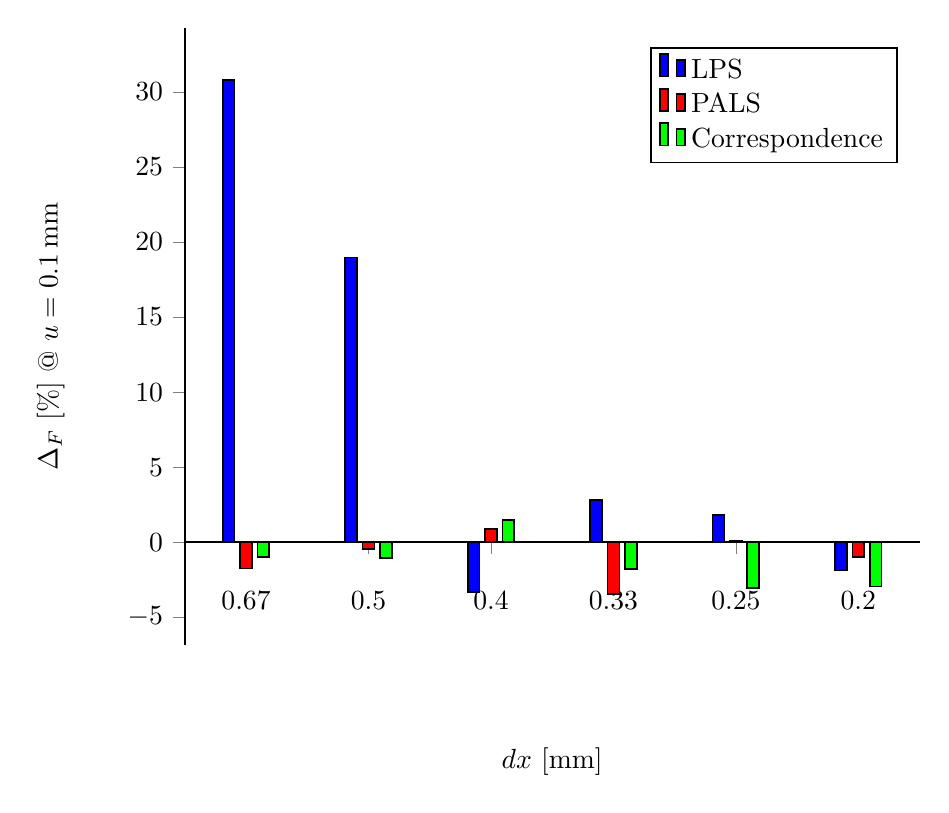
\begin{tikzpicture}
        \begin{axis}[
          symbolic x coords={
            0.67,
            0.5,
            0.4,
            0.33,
            0.25,
            0.2
          },
          ybar,%=0,
          bar width={0.15cm},
          width=0.9\linewidth,
          xtick=data,
          tick align=outside,
          axis x line*=middle,%left
          axis y line*=left,
          %x tick label style={yshift={-mod(\ticknum,2)*1em}},
          x tick label style={yshift={-1em}},
          label style={font=\figurefontsize},
          x label style={at={(axis description cs:0.5,-0.15)},anchor=north},
          y label style={at={(axis description cs:-0.15,.5)},anchor=south},%,rotate=90
          xlabel={$dx$ $[\si{\milli\meter}]$},
          ylabel={$\Delta_F$ $\left[\si{\percent}\right]$ @ $u=\SI{0.1}{\milli\meter}$},
          ticklabel style={font=\figurefontsize},
          legend cell align=left,
          legend pos=north east,
          legend style={font=\figurefontsize},
          %xmajorgrids,
          %after end axis/.code={
          %  \draw ({rel axis cs:0,0}|-{axis cs:0,0}) -- ({rel axis cs:1,0}|-{axis cs:0,0});
          %}
        ]
          \addplot[fill=blue] coordinates {
            (0.67,30.81)
            (0.5,18.97)
            (0.4,-3.34)
            (0.33,2.82)
            (0.25,1.82)
            (0.2,-1.89)
          };
          \addlegendentry{LPS}
          \addplot[fill=red] coordinates {
            (0.67,-1.77)
            (0.5,-0.45)
            (0.4,0.87)
            (0.33,-3.44)
            (0.25,0.11)
            (0.2,-1.01)
          };
          \addlegendentry{PALS}
          \addplot[fill=green] coordinates {
            (0.67,-1.00)
            (0.5,-1.07)
            (0.4,1.48)
            (0.33,-1.81)
            (0.25,-3.04)
            (0.2,-2.96)
          };
          \addlegendentry{Correspondence}
          
          %\draw ({rel axis cs:0,0}|-{axis cs:0,0}) -- ({rel axis cs:1,0}|-{axis cs:0,0});
          %\draw (rel axis cs:0,0) -- (rel axis cs:1,0);
          %\draw (axis cs:\pgfkeysvalueof{/pgfplots/xmin},0) -- (axis cs:\pgfkeysvalueof{/pgfplots/xmax},0);
        \end{axis}
      \end{tikzpicture}
      \tikzexternaldisable
    }
  \end{column}
\end{columns}

\end{frame}

\begin{frame}[t]{\secname}{\subsecname{} - Stiffness}

\begin{itemize}
  \item $\mbox{Convergence}=f\left(dx,\delta,\mbox{Material formulation}\right)$
  \item<2-> LPS material in Peridigm: no surface correction
  \only<2->{
    \begin{itemize}[noitemsep]
      \item Results $dx\ge\frac{t}{4}$ and $\delta>\SI{1}{mm}$ $\rightarrow$ ``all surface families''
      \item No family without effect of missing surface correction $\rightarrow$ Results not viable
      \item $dx$ and $\delta$ so that majority of families without influence of surface correction $\rightarrow$ Computational expense?!
    \end{itemize}
  }
  \only<2->{
  \item<2-> Correspondence materials:
    \begin{itemize}[noitemsep]
      \item Viable option
      \item Numerical problems $\rightarrow$ 3 non-collinear bonds must remain in family
      \item Hourglassing problematic
    \end{itemize}
  }
  \item<2-> Position-aware models $\rightarrow$ promising
  %\item Stiffness below CM for smallest element sizes $\rightarrow$ ``Real'' convergence might lie at even smaller element sizes \& horizons after dip
\end{itemize}

\end{frame}
\subsection{Failure}
\begin{frame}[t]{\secname}{\subsecname{}}

% Styles
\tikzset{
  failurespy style/.style={
    spy scope={%
      failurespyscope style,%
    },
    connect spies/.style={
      failurespyconnect style,%
    },
  }
}

\tikzset{
  failurespyscope style/.style={
    magnification=4,
    connect spies,                            % Connect orig. & detail
    width=0.45\linewidth,                     % Spy width
    height=0.40\linewidth,                    % Spy height
    every spy on node/.style={                % Source
      rectangle,                              % Form
      rounded corners=0.004\linewidth,        % Edge shape
      dashed,                                 % Dashed line
      draw=black,                             % Line color
      %thick,                                  % Line style for spy
    },
    every spy in node/.style={                % Spy
      rectangle,                              % Form
      rounded corners=0.004\linewidth,        % Edge shape
      dashed,                                 % Dashed line
      draw=black,                             % Line color
      %thick,                                  % Line style for spy
    },
  },
}

\tikzset{
  failurespyconnect style/.style={
    spy connection path={
      \draw[%
        %thick,
        dashed,
        black
      ] (tikzspyonnode) -- (tikzspyinnode); % In-On-Connection
    },
  },
}

\begin{columns}[t]
  \begin{column}{0.5\textwidth}
    \begin{itemize}
      \item Bond-based critical stretch models: \\[0.5ex]
      \begingroup
      \small 
        \begin{tabular}{@{}lc@{}}
          $\epsilon_{c}=\sqrt{\dfrac{5G_c}{9K\delta}}$&\cite{SillingSA2005,BobaruF2017}\\[2ex]%\tabto{5.5cm}
          $\epsilon_{c}=\sqrt{\dfrac{G_c}{\left[3G+\left(\frac34\right)^4\left(K-\frac{5G}{3}\right)\right]\delta}}$&\cite{MadenciE2014}%\tabto{5.5cm}
        \end{tabular}
      \endgroup
      \item<1-> Based on Griffith for existing pre-crack
      \item<1-> $\epsilon_{c}=f\left(\delta^{-\frac12}\right)$
      \item<2-> Reproducibility for various $\delta$ and adapted $\epsilon_c$ in SB-PD 1D-case for no pre-crack?%of failure displacement
      
    \end{itemize}
  \end{column}
  \begin{column}{0.5\textwidth}
    \only<3-4|handout:1-2>{
      \begin{block}{Hex, $dx=\SI{0.4}{\milli\meter}$}
        \only<3|handout:1>{
          % Data
          \pgfplotstableread[col sep=comma]{\materialpath/Data/Numerics/Hex_0-4_CritStretch.csv}{\loadedtable}
          % Dimensions
          \setlength{\figwidth}{\linewidth}
          \setlength{\figheight}{0.75\textheight}
          % Chart
          \tikzexternalenable
          \tikzsetnextfilename{Hex_0-4_CritStretch}
          \begin{tikzpicture}
            \begin{axis}[
              height=\figheight,
              width=\figwidth,
              axis lines=middle,
              cycle list name=color list,%linestyles*,
              cycle list shift=1,
              xmin=0,
              ymin=0,
              title=\empty,
              xlabel={$u$ $[\si{\milli\meter}]$},
              ylabel={$F$ $[\si{\newton}]$},
              label style={font=\figurefontsize},
              %x label style={at={(axis description cs:0.5,-0.075)},anchor=north},
              %y label style={at={(axis description cs:-0.085,0.5)},rotate=90,anchor=south},
              legend pos=south west,
              legend cell align={left},
              legend style={font=\figurefontsize},
              ticklabel style={font=\figurefontsize},
            ]%   each nth point={2}
    %           %\addplot+ table[x=Dx5, y=Fx5] {\loadedtable};
    %           %\addlegendentry{$\delta=\SI{5}{\milli\meter}$, $\epsilon_c=\num[round-mode=places,round-precision=2]{9.797959e-3}$}
    %           %\addplot+ [] table[x=Dx4, y=Fx4] {\loadedtable};
    %           %\addlegendentry{$\delta=\SI{4}{\milli\meter}$, $\epsilon_c=\num[round-mode=places,round-precision=2]{1.0954451e-2}$}
              \addplot+ [] table[x=Dx3, y=Fx3] {\loadedtable};
              \addlegendentry{$\delta=\SI{3}{\milli\meter}$}%, $\epsilon_c=\num[round-mode=places,round-precision=2]{1.2649111e-2}$}
              \addplot+ [] table[x=Dx2, y=Fx2] {\loadedtable};
              \addlegendentry{$\delta=\SI{2}{\milli\meter}$}%, $\epsilon_c=\num[round-mode=places,round-precision=2]{1.5491933e-2}$}
              \addplot+ [] table[x=Dx1.5, y=Fx1.5] {\loadedtable};
              \addlegendentry{$\delta=\SI{1.5}{\milli\meter}$}%, $\epsilon_c=\num[round-mode=places,round-precision=2]{1.7888544e-2}$}
    %           \pgfplotsset{cycle list shift=2} % Jump one in cycle - 1.25
              \addplot+ [] table[x=Dx1.2, y=Fx1.2] {\loadedtable};
              \addlegendentry{$\delta=\SI{1.2}{\milli\meter}$}%, $\epsilon_c=\num[round-mode=places,round-precision=2]{2e-2}$}
              \pgfplotsset{cycle list shift=1} % Jump one in cycle - 1.18
              \addplot+ [] table[x=Dx1, y=Fx1] {\loadedtable};
              \addlegendentry{$\delta=\SI{1}{\milli\meter}$}%, $\epsilon_c=\num[round-mode=places,round-precision=2]{2.1908902e-2}$}
              \addplot+ [] table[x=Dx0.875, y=Fx0.875] {\loadedtable};
              \addlegendentry{$\delta=\SI{0.875}{\milli\meter}$}%, $\epsilon_c=\num[round-mode=places,round-precision=2]{2.3421602e-2}$}
            \end{axis}
          \end{tikzpicture}
          \tikzexternaldisable
%             \includegraphics[width=\figwidth,height=\figheight,keepaspectratio]{example-image-a}           
        }
        \only<4|handout:2>{
          \setlength{\figheight}{0.55\textheight}
          \vspace{1ex}
          \figurefontsize
          \begin{minipage}[t][0.65\textheight][t]{0.49\linewidth}
            \centering
            \tikzexternalenable
            \tikzsetnextfilename{PD_Hex_Damage_0-4_1-2_3630_-z_spy}
            \begin{tikzpicture}[
              failurespy style,
            ]
              \node[inner sep=0] (PDHex1) {\includegraphics[angle=90,width=\linewidth,height=\figheight,keepaspectratio]{PD_Hex_Damage_0-4_1-2_3630_-z_ct.png}};
              \begin{scope}[
                shift={(PDHex1.south west)},
                x={(PDHex1.south east)},
                y={(PDHex1.north west)},
              ]
                \coordinate (spypointpdhex1) at (0.5,0.275);
                \coordinate (spyviewerpdhex1) at (1.0,0.5);
                \spy on (spypointpdhex1) in node[anchor=west] at (spyviewerpdhex1);
              \end{scope}
            \end{tikzpicture}\\
            \tikzexternaldisable
            $\delta=\SI{1.2}{\milli\meter}$
          \end{minipage}
          \begin{minipage}[t][0.65\textheight][t]{0.49\linewidth}
            \centering
            \tikzexternalenable
            \tikzsetnextfilename{PD_Hex_Damage_0-4_2_3955_-z_spy}
            \begin{tikzpicture}[
              failurespy style,
            ]
              \node[inner sep=0] (PDHex2) {\includegraphics[angle=90,width=\linewidth,height=\figheight,keepaspectratio]{PD_Hex_Damage_0-4_2_3955_-z_ct.png}};
              \begin{scope}[
                shift={(PDHex2.south west)},
                x={(PDHex2.south east)},
                y={(PDHex2.north west)},
              ]
                \coordinate (spypointpdhex2) at (0.5,0.67);
                \coordinate (spyviewerpdhex2) at (1.0,0.5);
                \spy on (spypointpdhex2) in node[anchor=west] at (spyviewerpdhex2);
              \end{scope}
            \end{tikzpicture}\\
            \tikzexternaldisable
            $\delta=\SI{2}{\milli\meter}$
          \end{minipage}
        }
      \end{block}
    }
    \only<5-|handout:3>{
      \begin{block}{Tet, $dx=\SI{0.5}{\milli\meter}$}
        %\only<3|handout:0>{
          \setlength{\figheight}{0.55\textheight}
          \vspace{1ex}
          \figurefontsize
          \begin{minipage}[t][0.65\textheight][t]{0.49\linewidth}
            \centering
            \tikzexternalenable
            \tikzsetnextfilename{PD_Tet_Damage_0-5_0-5625_9600_-z_spy}
            \begin{tikzpicture}[
              failurespy style,
            ]
              \node[inner sep=0] (PDTet1) {\includegraphics[angle=90,width=\linewidth,height=\figheight,keepaspectratio]{PD_Tet_Damage_0-5_0-5625_9600_-z_ct.png}};
              \begin{scope}[
                shift={(PDTet1.south west)},
                x={(PDTet1.south east)},
                y={(PDTet1.north west)},
              ]
                \coordinate (spypointpdtet1) at (0.5,0.700);
                \coordinate (spyviewerpdtet1) at (1.0,0.5);
                \spy on (spypointpdtet1) in node[anchor=west] at (spyviewerpdtet1);
              \end{scope}
            \end{tikzpicture}\\
            \tikzexternaldisable
            $\delta=\SI{0.56}{\milli\meter}$
          \end{minipage}
          \begin{minipage}[t][0.65\textheight][t]{0.49\linewidth}
            \centering
            \tikzexternalenable
            \tikzsetnextfilename{PD_Tet_Damage_0-5_1-5_1830_-z_spy}
            \begin{tikzpicture}[
              failurespy style,
            ]
              \node[inner sep=0] (PDTet2) {\includegraphics[angle=90,width=\linewidth,height=\figheight,keepaspectratio]{PD_Tet_Damage_0-5_1-5_1830_-z_ct.png}};
              \begin{scope}[
                shift={(PDTet2.south west)},
                x={(PDTet2.south east)},
                y={(PDTet2.north west)},
              ]
                \coordinate (spypointpdtet2) at (0.5,0.300);
                \coordinate (spyviewerpdtet2) at (1.0,0.5);
                \spy on (spypointpdtet2) in node[anchor=west] at (spyviewerpdtet2);
              \end{scope}
            \end{tikzpicture}\\
            \tikzexternaldisable
            $\delta=\SI{1.5}{\milli\meter}$
          \end{minipage}
        %}
      \end{block}
    }
  \end{column}
\end{columns}

\end{frame}
\begin{frame}[t]{\secname}{\subsecname{}}

\begin{itemize}
  \item No
  \item Assumption of pre-crack not met
  \item Equality of Griffith-based relationship between critical stretch, strain energy release rate, bulk modulus \& horizon not met
  \item Unphysical damage shapes for larger horizons $\rightarrow$ effect of missing surface correction in material model
  \item Energy-based failure criterion?
\end{itemize}

\end{frame}

\subsection{Stochastics}
\begin{frame}[t]{\secname}{\subsecname{} - Why \& Implementation}

\begin{itemize}
  \item Ensure effect causing failure adequately described \& robust solution
  %\item Check solution dependency on underlying discretization scheme
  \item Prove influence on damage of
  \begin{itemize}[noitemsep]
    \item Scatter in stress-strain-curves, micro-voids \& findings in micrographs
    \item Varying degree of cure, disparities from machining
  \end{itemize}
\end{itemize}

\setlength{\figheight}{0.475\textheight}
\begin{columns}[t]
  \begin{column}{0.5\textwidth}
    \only<2->{
      \begin{block}{Stochastic model}
        \centering
        % Variables
        \def\nb{20}
        \def\ne{10}
        % Picture
        \tikzexternalenable
        \tikzsetnextfilename{Implementation_Stochastic_Constant}
        \begin{tikzpicture}
  \begin{axis}[
    width=\linewidth,
    height=\figheight,
    ybar,
    bar shift=0pt,
    %axis lines=middle,
    axis x line=bottom,
    axis y line=middle,
    samples=10,
    enlarge y limits=upper,
    xmin=-\ne/2-0.75,
    xmax= \ne/2+0.75,
    ymin=0,
    ymax=(\nb+1)*1.05,
    xlabel=$K$,
    ylabel=$n_e$,
    x label style={at={(axis description cs:1.0,0.0)},anchor=south west},
    y label style={at={(axis description cs:0.5,1.0)},anchor=south west},
    %xtick={-\ne/2,0,\ne/2},
    xtick={-5,0,5},
    ymajorticks=false,
    xticklabels={$\bar{K}-\Delta$,$\bar{K}$,$\bar{K}+\Delta$},
    yticklabels={},
  ]
    %\addplot +[black,fill=gray]{rnd};
    %\addplot coordinates {(-\ne/2,\nb)};
    \foreach \x in {-5,-4,...,5} {
      \addplot+[black,fill=gray] coordinates {(\x,\nb+rand)};%,bar shift=0.5
    }
  \end{axis}
\end{tikzpicture}
        \tikzexternaldisable
      \end{block}
    }
  \end{column}
  \begin{column}{0.5\textwidth}
    \only<3->{
      \begin{block}{Base FE model}
        \centering
        \includegraphics[width=0.85\linewidth,height=\figheight,keepaspectratio]{Model_FE_Hex_0-5_Stochastic_ct}
      \end{block}
    }
  \end{column}
\end{columns}
  
\end{frame}


% \begin{figure}[htbp]
%   \setlength{\figheight}{5cm}
%   \begin{subfigure}{0.49\linewidth}
%     \begin{minipage}[b][\figheight]{\linewidth}
%       \centering
%       % Variables
%       \def\nb{20}
%       \def\ne{10}
%       % Picture
%       \begin{tikzpicture}
  \begin{axis}[
    width=\linewidth,
    height=\figheight,
    ybar,
    bar shift=0pt,
    %axis lines=middle,
    axis x line=bottom,
    axis y line=middle,
    samples=10,
    enlarge y limits=upper,
    xmin=-\ne/2-0.75,
    xmax= \ne/2+0.75,
    ymin=0,
    ymax=(\nb+1)*1.05,
    xlabel=$K$,
    ylabel=$n_e$,
    x label style={at={(axis description cs:1.0,0.0)},anchor=south west},
    y label style={at={(axis description cs:0.5,1.0)},anchor=south west},
    %xtick={-\ne/2,0,\ne/2},
    xtick={-5,0,5},
    ymajorticks=false,
    xticklabels={$\bar{K}-\Delta$,$\bar{K}$,$\bar{K}+\Delta$},
    yticklabels={},
  ]
    %\addplot +[black,fill=gray]{rnd};
    %\addplot coordinates {(-\ne/2,\nb)};
    \foreach \x in {-5,-4,...,5} {
      \addplot+[black,fill=gray] coordinates {(\x,\nb+rand)};%,bar shift=0.5
    }
  \end{axis}
\end{tikzpicture}
%     \end{minipage}
%     \caption{Simple stochastic model}
%     \label{fig:Thry:Stochastic:Distribution}
%   \end{subfigure}
%   \hfill
%   \begin{subfigure}{0.49\linewidth}
%     \begin{minipage}[b][\figheight]{\linewidth}
%       %\includegraphics[width=\linewidth,height=\figheight,keepaspectratio]{../../Material/Figures/Model_FE_Hex_0-5_Stochastic_ct.png}
%       \includegraphics[width=\linewidth,height=\figheight,keepaspectratio]{Model_FE_Hex_0-5_Stochastic_ct}
%     \end{minipage}
%     \caption{Base FE mesh with stochastic block distribution}
%     \label{fig:Thry:Stochastic:FEModel}
%   \end{subfigure}
%   \caption{Implementation of stochastic material distribution for PD simulations}
%   \label{fig:Thry:Stochastic:Implementation}
% \end{figure}
\begin{frame}[t]{\secname}{\subsecname}
  
\begin{itemize}
  \item Hex: $dx=\SI{0.4}{\milli\meter}$, $\delta=\SI{1.2}{\milli\meter}$
\end{itemize}

\begin{columns}[t]
  \begin{column}{0.375\textwidth}
    \only<1->{
      \begin{block}{Force-Displacement plot}
        \centering
        % Size
        \setlength{\figheight}{0.75\textheight}
        % Data
        \pgfplotstableread[col sep=comma]{\materialpath/Data/Numerics/Hex_0-4_1-2_Stoch.csv}{\loadedtable}
        % Chart
        \tikzexternalenable
        \tikzsetnextfilename{Hex_0-4_1-2_Stoch}
        \begin{tikzpicture}
          \begin{axis}[
            %height=\figheight+\baselineskip,
            height=\figheight,
            width=\linewidth,
            axis lines=middle,
            cycle list name=color list,%linestyles*,
            %cycle list shift=1,
            xmin=0,
            ymin=0,
            title=\empty,
            %xlabel={Displacement $[\si{\milli\meter}]$},
            %ylabel={Force $[\si{\newton}]$},
            xlabel={$u$ $[\si{\milli\meter}]$},
            ylabel={$F$ $[\si{\newton}]$},
            %x label style={at={(axis description cs:0.5,-0.075)},anchor=north},
            %y label style={at={(axis description cs:-0.105,0.5)},rotate=90,anchor=south},
            label style={font=\figurefontsize},
            %legend pos=south west,
            legend cell align={left},
            legend style={
              font=\figurefontsize,
              at={(0.025,0.85)},
              anchor=north west,
            },
            ticklabel style={font=\figurefontsize},
          ]%   each nth point={2}
            \addplot+ [thick] table[x=DxNo, y=FxNo] {\loadedtable};
            \addlegendentry{No stochastics}
            \addplot+ [] table[x=DxSto1, y=FxSto1] {\loadedtable};
            \addlegendentry{Stochastic 1}
            \addplot+ [] table[x=DxSto2, y=FxSto2] {\loadedtable};
            \addlegendentry{Stochastic 2}
            \addplot+ [] table[x=DxSto3, y=FxSto3] {\loadedtable};
            \addlegendentry{Stochastic 3}
          \end{axis}
        \end{tikzpicture}
        \tikzexternaldisable
      \end{block}
    }
  \end{column}
  \begin{column}{0.625\textwidth}
    \only<2->{
      \begin{block}{Failure patterns}
        \setlength{\figheight}{0.625\textheight}
        \figurefontsize
        \begin{tabular}{@{}c@{}c@{}c@{}c@{}c@{}}
        \begin{minipage}[t][\figheight]{0.1925\linewidth}
          \centering
          \includegraphics[angle=90,width=\linewidth,height=\figheight,keepaspectratio]{PD_Hex_Damage_0-4_1-2_3630_-z_ct}
        \end{minipage}
        &
        \begin{minipage}[t][\figheight]{0.1925\linewidth}
          \centering
          \includegraphics[angle=90,width=\linewidth,height=\figheight,keepaspectratio]{PD_Hex_Stoch_1_Damage_0-4_1-2_3475_-z_ct}
        \end{minipage}
        &
        \begin{minipage}[t][\figheight]{0.1925\linewidth}
          \centering
          \includegraphics[angle=90,width=\linewidth,height=\figheight,keepaspectratio]{PD_Hex_Stoch_2_Damage_0-4_1-2_3540_-z_ct}
        \end{minipage}
        &
        \begin{minipage}[t][\figheight]{0.1925\linewidth}
          \centering
          \includegraphics[angle=90,width=\linewidth,height=\figheight,keepaspectratio]{PD_Hex_Stoch_3_Damage_0-4_1-2_3292_-z_ct}
        \end{minipage}
        &
        \begin{minipage}[t][\figheight]{0.1925\linewidth}
          \centering
          \includegraphics[angle=90,width=\linewidth,height=\figheight,keepaspectratio]{KrauseD_Damage_LY564_statisch}
        \end{minipage}\\
        No & 1 & 2 & 3 & \cite{KrauseD2016}
        \end{tabular}
      \end{block}
    }
  \end{column}
\end{columns}

\end{frame}

\input{Slides/Slide_Results_Stochastics_Tet}

\section{Conclusion}
\begingroup
\slidenumberfreeheader
        
% \frame[noframenumbering]{
\begin{frame}<handout:0>[noframenumbering]
  %\tableofcontents[currentsection,subsectionstyle=hide]
  \tableofcontents[currentsection,hideothersubsections]
%   \begin{minipage}[t][0.8\textheight]{\textwidth}
%     \tableofcontents[
%       currentsection,
%       sectionstyle=show/show,
%       subsectionstyle=show/show/hide
%     ]
%   \end{minipage}
%   \hfill
% }
\end{frame}

\endgroup
\begin{frame}[t]{\secname}%{\subsecname}
  
\begin{itemize}
  \only<1->{
    \item Discretization:
      \begin{itemize}[noitemsep]
        \item Influence of base discretization
        \item Entropy in tet mesh benefitial
      \end{itemize}
  }
  \only<2->{
    \item Convergence:
      \begin{itemize}[noitemsep]
        \item Discontinuous
        \item $m\approx3$ for hex \& $m\approx1.1$ for tet mesh best values $\leftrightarrow$ FEM for tension
      \end{itemize}
  }
  \only<3->{
    \item Failure:
      \begin{itemize}[noitemsep]
        \item Bond-based critical stretch criterion not suitable in state-based materials
        \item Energy-based criterion required
      \end{itemize}
  }
  \only<4->{
    \item Stochastics:
      \begin{itemize}[noitemsep]
        \item Suitable method to check model robustness
        \item Increases entropy in hex mesh, effect smaller for tet mesh
      \end{itemize}
  }
\end{itemize}

\end{frame}

\begin{frame}[fragile,t]{\secname}%{\subsecname}

\begin{itemize}
 \item RVE: Initial attempt with tet mesh and critical stretch model
\end{itemize}

% \begin{center}
\begin{minipage}[t][0.7\textheight][t]{0.49\textwidth}
  \centering
  \IfFileExists{Videos/RVE_Fatigue_r113360_dam_R3_nolegend.mp4}{
  \only<1|handout:0>{
		\begin{tikzpicture}
		  % Axis style
		  \pgfplotsset{
			myperidigmdamageaxis style/.style={
			  hide axis,
			  scale only axis,
			  point meta min=0.0,                       % Minimum value colorbar
			  point meta max=0.5,                       % Maximum value colorbar
			  tick label style={font=\figurefontsize},  
			  %colormap/bluered,                         % Colormap preset
			}
		  }
		  % Video
		%   \begin{pgfonlayer}{layervideo}
		%     \node (video) {
		%       \includemedia[
		%         height=0.7\textheight,
		%         width=0.9\textwidth,
		%         keepaspectratio,
		%         activate=pageopen,
		%         addresource=Videos/RVE_Fatigue_r113360_udam_R3.mp4,
		%         flashvars={source=Videos/RVE_Fatigue_r113360_udam_R3.mp4}
		%         ]{}{VPlayer.swf}%{VPlayer9.swf}
		%     };
			\node (video1) {
			  \includemedia[
				height=0.65\textheight,
				width=0.7\linewidth,
				keepaspectratio,
				activate=pageopen,
				addresource=Videos/RVE_Fatigue_r113360_dam_R3_nolegend.mp4,
				flashvars={source=Videos/RVE_Fatigue_r113360_dam_R3_nolegend.mp4}
				]{}{VPlayer.swf}%{VPlayer9.swf}
			};
		  % Colorbar right
			\begin{axis}[%
			  myperidigmdamageaxis style,
	  %         %at={(video.east)},
	  %         %anchor=west,
			  at={(video1.west)},
			  anchor=east,
			  height=0.65\textheight,
			  xshift=3.0cm,                              % Adjust this for horizontal sep
			  colorbar left,                             % Activate colorbar
			  colorbar sampled,
			  colormap name=paraviewblueredcolormap,
			  colorbar style={
				paraviewdiscrete256colorbar style,
				%ylabel=Damage variable [-],             % Label
				ylabel=Damage [-],                       % Label
				y label style={
				  at={(2em,1.075)},
				  rotate=-90,
				},
				label style={font=\figurefontsize},
				scaled y ticks=false,
			  },
			]
			  \addplot [draw=none] coordinates {(0,0)}; % Dummy plot
			\end{axis}
		\end{tikzpicture}
	  }
	  \only<2|handout:1>{
		\hspace{2em}
		\includegraphics[width=\linewidth,height=0.65\textheight,keepaspectratio]{PD_RVE_Fatigue_r113360_dam_R3_nolegend_2400_1000px_ct.png}
	  }
	}{
	  \only<1|handout:1>{
		\hspace{2em}
		\includegraphics[width=\linewidth,height=0.65\textheight,keepaspectratio]{PD_RVE_Fatigue_r113360_dam_R3_nolegend_2400_1000px_ct.png}
	  }
	
	}
\end{minipage}
\begin{minipage}[t][0.7\textheight][t]{0.49\textwidth}
  \IfFileExists{Videos/RVE_Fatigue_r113360_dam_R3_nolegend.mp4}{
	  %\includegraphics[width=\linewidth]{example-image-a}
	  \only<1|handout:0>{
		\begin{tikzpicture}
		  % Axis style
		  \pgfplotsset{
			mydisplacementaxis style/.style={
			  hide axis,
			  scale only axis,
			  point meta min=0.0,                       % Minimum value colorbar
			  point meta max=0.04,                       % Maximum value colorbar
			  tick label style={font=\figurefontsize},  
			  %colormap/bluered,                         % Colormap preset
			  %colorbar sampled,                         % Steps in colorbar
			}
		  }
		  % Layers
		%   \pgfdeclarelayer{layervideo}
		%   \pgfdeclarelayer{layercolorbar}
		%   \pgfsetlayers{layervideo,layercolorbar}
		  % Video
		%     \node (video) {
		%       \includemedia[
		%         height=0.7\textheight,
		%         width=0.9\textwidth,
		%         keepaspectratio,
		%         activate=pageopen,
		%         addresource=Videos/RVE_Fatigue_r113360_udam_R3.mp4,
		%         flashvars={source=Videos/RVE_Fatigue_r113360_udam_R3.mp4}
		%         ]{}{VPlayer.swf}%{VPlayer9.swf}
		%     };
			\node (video2) {
			  \includemedia[
				height=0.65\textheight,
				width=0.7\linewidth,
				keepaspectratio,
				activate=pageopen,
				addresource=Videos/RVE_Fatigue_r113360_u_R3_nolegend.mp4,
				flashvars={source=Videos/RVE_Fatigue_r113360_u_R3_nolegend.mp4}
				]{}{VPlayer.swf}%{VPlayer9.swf}
			};
		  % Colorbar right
			\begin{axis}[%
			  mydisplacementaxis style,
			  %at={(video.east)},
			  %anchor=west,
			  at={(video2.east)},
			  anchor=west,
			  height=0.65\textheight,
			  xshift=-3.0cm,
			  colorbar right,                           % Activate colorbar
			  colorbar sampled,
			  colormap name=paraviewblueredcolormap,
			  colorbar style={
				paraviewdiscrete256colorbar style,
				%ylabel=Damage variable [-],             % Label
				ylabel={$u_y$ $\si{\milli\meter}$},      % Label
				y label style={
				  at={(-1em,1.075)},
				  rotate=-90,
				},
				label style={font=\figurefontsize},
				yticklabel style={
				  /pgf/number format/fixed,
				  /pgf/number format/precision=2,
				},
				scaled y ticks=false,
			  },
			]
			  \addplot [draw=none] coordinates {(0,0)}; % Dummy plot
			\end{axis}
		\end{tikzpicture}
	  }
	  \only<2|handout:1>{
		\includegraphics[width=\linewidth,height=0.65\textheight,keepaspectratio]{Exp_Matrix_Failure}
	  }
	}{
	  \only<1|handout:1>{
		\includegraphics[width=\linewidth,height=0.65\textheight,keepaspectratio]{Exp_Matrix_Failure}
	  }
	}
\end{minipage}

% \end{center}

\end{frame}


\begingroup
\slidenumberfreeheader

\begin{frame}[noframenumbering]

\vfill
\begingroup
\centering
\huge Thank you for your attention.
\endgroup
\vfill

\begin{block}{Contact}
\vspace{1ex}
{\footnotesize
\begin{tabularx}{\linewidth}{lXl@{\hskip 0.5em}X}
\usebeamertemplate{itemize item}{}	& \multicolumn{3}{l}{Christian Willberg}	\\
		& \multicolumn{3}{l}{German Aerospace Center}	\\
		& \multicolumn{3}{l}{Institute of Composite Structures and Adaptive Systems}	\\
		& \multicolumn{3}{l}{Department of Structural Mechanics}	\\[1ex]
		& Lilienthalplatz 7	& \phone	& +49 (0)531 295-2489 	\\
		& 38108 Braunschweig	& \Faxmachine	& +49 (0)531 295-2232	\\
		& Germany		& \Letter	& \href{mailto:christian.willberg@dlr.de}{christian.willberg@dlr.de}	\\
		& 			& \Mundus	& \href{http://www.dlr.de/fa}{www.dlr.de/fa}	\\
\end{tabularx}
}
\end{block}

% \begin{block}{\LaTeX-Template source}
% {\footnotesize
% \href{http://teamsites.dlr.de/rm/latex/SitePages/Homepage.aspx}{http://teamsites.dlr.de/rm/latex/SitePages/Homepage.aspx}
% }
% \end{block}
\end{frame}
\endgroup
{
\begingroup
\slidenumberfreeheader

\begin{frame}[noframenumbering]{Bibliography}

\begingroup
\renewcommand*{\bibfont}{\footnotesize} % for biblatex package
\printbibliography
\endgroup

% \begin{block}{\LaTeX-Template source}
% {\footnotesize
% \href{http://teamsites.dlr.de/rm/latex/SitePages/Homepage.aspx}{http://teamsites.dlr.de/rm/latex/SitePages/Homepage.aspx}
% }
% \end{block}
\end{frame}
\endgroup
}

\end{document}
